\documentclass[a4,center,fleqn]{NAR}

% Enter dates of publication
\copyrightyear{2009}
\pubdate{31 July 2009}
\pubyear{2009}
\jvolume{37}
\jissue{12}


\usepackage{mathrsfs}
\usepackage{amsmath, bm}


\newcommand{\pois}{\text{Poisson}}
\newcommand{\OurMethod}{MEACA}
\newcommand{\HowmanyTest}{six}
\newcommand{\aaCase}{a}
\newcommand{\aCase}{c}
\newcommand{\cCase}{b}
\newcommand{\eCase}{d}
\newcommand{\fCase}{e}
\newcommand{\CMR}{CAMERA-rank}
\newcommand{\CMT}{CAMERA-modt}
\newcommand{\gent}{SigPathway}
\newcommand{\gen}{geneSetTest}
\newcommand{\genr}{MRGSE}
\newcommand{\thepapertobefinished}{Zhuo, Jiang and Di, unpublished work}
\newcommand{\HowmanySimu}{$10,000$}
\newcommand{\FDR}{Benjamini-Hochberg}
\newcommand{\FDRabb}{BH}
\newcommand{\cov}{\text{Cov}}
\newcommand{\cor}{\text{Corr}}
\newcommand{\var}{\text{Var}}
\newcommand{\DED}{differentially expressed}

%\newcolumntype{M}[1]{>{\centering\arraybackslash}m{#1}}
%%%%%%%%%%%%%%%%%%%%%%%%%%%%%%%%%%%%%%%%%%%%%%%%%
%
%\setcounter{footnote}{2}
%
%\title[This is an Example of Recto Running Head]{Accounting for correlations in competitive gene set
%	test for improved interpretation of genome-scale data}
%
%\author{Bin Zhuo$^{*}$\email{zhuob@oregonstate.edu} \\
%	Department of Statistics, Oregon State University, Corvallis, OR, 97333
%	\and 
%	Duo Jiang$^{*}$\email{jiangd@stat.oregonstate.edu}\\
%	Department of Statistics, Oregon State University, Corvallis, OR, 97333
%}



\begin{document}
	
	
	\title{Accounting for correlations in competitive gene set
		test for improved interpretation of genome-scale data}
	
	\author{%
		Bin Zhuo\,$^{1}$,
		Duo Jiang\,$^{2}$
	%	and Second Co-Author\,$^2$%
		\footnote{To whom correspondence should be addressed.
			Tel: +44 000 0000000; Fax: +44 000 0000000; Email: jiangd@oregonstate.edu}}
	
	\address{%
	%	$^{1, 2}$Department of Statistics, Oregon State University, 239 Weniger Hall, Corvallis, OR, 97333, USA\\
		$^{1, 2}$Department of Statistics, Oregon State University, 239 Weniger Hall, Corvallis, 
		OR, 97331, USA}
	% Affiliation must include:
	% Department name, institution name, full road and district address,
	% state, Zip or postal code, country
	
	\history{%
		Received January 1, 20XX;
		Revised February 1, 20XX;
		Accepted March 1, 20XX}
	
	\maketitle
	
	%\date{{\it Received October} 2004. {\it Revised February} 2005.\newline 
	%{\it Accepted March} 2005.}
	
	%\pagerange{\pageref{firstpage}--\pageref{lastpage}} \pubyear{2006}
	
	%\volume{59}
	%\artmonth{December}
	%\doi{10.1111/j.1541-0420.2005.00454.x}
	
	%  This label and the label ``lastpage'' are used by the \pagerange
	%  command above to give the page range for the article
	
%	\label{firstpage}
	
	%  pub the summary here
	
	\begin{abstract}
	Competitive gene-set analysis is a widely used tool for interpreting high-throughput biological 
	data, such as gene expression and proteomics data. It aims at testing a known category of genes 
	for enriched association signals in a list of genes inferred from genome-wide data. Most 
	conventional enrichment testing methods ignore or do not properly account for the widespread 
	correlations among genes, which, as we show, can result in mis-calibrated type I error rates 
	and/or power loss. We propose a new framework, \OurMethod, for gene-set test based on a mixed 
	effects quasi-likelihood model, where the data are not required to be Gaussian. Our method 
	effectively adjusts for completely unknown,	unstructured correlations among genes. It uses a 
	score test approach and allows for analytical assessment of $p$-values. Compared to existing 
	methods such as GSEA and CAMERA, our method enjoys robust and substantially improved control 
	over type I error and maintains good power in a variety of correlation structure and 
	association settings. We also present two real data analyses to illustrate our approach.
	\end{abstract}
	
	%
	%  Please place your key words in alphabetical order, separated
	%  by semicolons, with the first letter of the first word capitalized,
	%  and a period at the end of the list.
	%
%	
%	\begin{keywords}
%		%Colostrum; Milk; Milk oligosaccharide; Non-human mammal.
%		mixed effects; quasi-likelihood; gene set test; correlation
%	\end{keywords}
%	
%	\maketitle
	
	\section{Introduction}\label{section:introduction}
	
\textit{Gene-set tests} (also called enrichment 
analysis in some literature) aim to evaluate  the association between the expression levels of 
genes in a pre-defined set, 
referred to as the test set, and experimental or environmental factors of interest.
It examines whether the test set is enriched (or depleted) with differential expression (DE) 
signals, where the DE signal of a gene can be quantified by comparing the gene's expression 
levels across treatment groups for the factor of interest. The test set could be a known 
pathway or given by a 
functional annotation term from a database such as KEGG \citep{kanehisa2000kegg} or GO 
\citep{ashburner2000gene}.
%	A key task of gene expression analysis involves the detection of differentially expressed 
%genes. Differential expression (DE) analysis  evaluates each individual gene separately, and 
%therefore it fails to provide insight into the relation between treatment variables and the 
%prior gene set under study. 
Gene-set tests help researchers understand the underlying biological processes in terms of 
ensembles of genes.

%	\textbf{What are the differences between self-contained and competitive test? And how does 
%they	work?}\\
Depending on the definition of the null hypothesis, there are two types of gene-set tests
\citep{goeman2007analyzing}: the \textit{self-contained} test and the \textit{competitive} 
test. A self-contained test examines the DE signals of genes in the test set without reference 
to other genes in the genome 	
\citep{goeman2005testing,goeman2004global,huang2013gene,tsai2009multivariate,wu2010roast}. A 
competitive test compares DE signals of genes in the test set to those of genes not in the test 
set \citep{tian2005discovering,wu2012camera,yaari2013quantitative}. Many methods, regardless of 
the type of test, perform a three-stage analysis
\citep{khatri2012ten}: at the first stage, a \textit{gene-level statistic} is calculated for 
each gene in the whole genome to measure the association between the expression profiles and the
experimental design variables; such gene-level statistics include, among others,
\textit{signal-to-noise ratio} \citep{subramanian2005gene}, \textit{ordinary $t$-statistic}
\citep{tian2005discovering} or \textit{moderated $t$-statistic} \citep{Smyth2004moderated},
\textit{log fold change} \citep{kim2005page} and \textit{$Z$-score} 
\citep{efron2007correlation}. At
the second stage, a \textit{set-level statistic} is obtained by utilizing the gene-level 
statistics
from the first stage and their membership with respect to the test set (i.e., whether the gene
belongs to the test set). Examples of the set-level statistics are \textit{enrichment score}
\citep{subramanian2005gene}, \textit{maxmean statistic} \citep{efron2007testing}, and a 
statistic derived from convoluted distribution of gene-level statistics 
\citep{yaari2013quantitative}, to name
a few. At the third stage, a $p$-value is assigned to the test set by comparing the set-level
statistic to its reference distribution. The competitive gene-set test is much more popular 
among genomic literature \citep{gatti2010heading,goeman2007analyzing}.  

%Competitive gene set test \citep{goeman2007analyzing} is a gene expression analysis that 
%compares
%differential expression (DE) for genes in the test set to that for genes not in the test set. 
%Most
%competitive gene set tests, as described by \cite{barry2008statistical}, are typically 
%two-stage
%procedures:  on the second stage, a $p$-value is reported from the The test set may represent
%biological pathways or network, or some other grouping based on biological knowledge. 
%Incorporating
%such prior information of the grouping makes it easier for biologists to interpret the results 
%of
%DE analysis.

%	\textbf{Independent gene set test} \\
Many competitive gene-set tests rely on independence between gene-level statistics, which 
implicitly requires independence among the expression level of different genes.
Examples of  independence-assuming gene-set tests include, among many others, PAGE 
\citep{kim2005page}, the 
contingency-table-based tests (see \citet{huang2009bioinformatics} 
for a review) and sigPathway\citep{Smyth2004moderated,tian2005discovering}. 
% Those tests are parametric or rank-based procedures
%that assume the gene-level statistics to be independent and identically distributed, or gene
%permutation procedures that generate the same approximate null for the set-level statistics. 
%For example, the PAGE \citep{kim2005page} conducts one-sample $z$-test by comparing the mean 
%of 
%gene-level statistics (i.e., the mean of log fold changes) in the test set to a normal 
%distribution under the null. The $2\times 2$ contingency-table-based tests examine the 
%significance of the test set by dichotomizing the outcomes of DE analysis and 
%cross-classifying 
%the genes according to whether they are indicated as DE and whether they are in the test set 
%(see \cite{huang2009bioinformatics} for a review and references therein). The sigPathway 
%\citep{tian2005discovering} and ``\gen" in the limma package \citep{Smyth2004moderated} 
%evaluate the set-level $p$-values by permuting gene labels. 
However, between-gene correlations can be widespread, for example, among co-regulated genes 
\citep{gatti2010heading}.  Even mild correlations may result in inflated false 
positive rate for independence-assuming gene-set tests 
\citep{efron2007testing,gatti2010heading,goeman2007analyzing, 
	wu2012camera,yaari2013quantitative}.

%	\textbf{Tests that account for inter-gene correlation}\\
A handful of methods have been proposed to account for between-gene correlations in competitive 
gene-set tests. One attempt is to evaluate the set-level statistic by permuting the biological 
sample labels \citep{efron2007testing,subramanian2005gene}. Permuting sample labels
does not require an explicit understanding of the underlying correlation structure among genes 
and thus protects the test against such correlations. Since permuting sample labels is 
computationally	inefficient, \citet{zhou2013empirical} proposed an analytic approximation to 
permutations for set-level score statistics, which preserves the essence of permutation 
gene-set analysis with greatly reduced computational burden. However, permuting sample labels 
in these methods inevitably alters the null and alternative hypotheses being tested, and 
therefore confuses the competitive test with the self-contained test, making the results hard 
to interpret \citep{goeman2007analyzing, khatri2012ten, wu2012camera}. Another attempt is to 
use set-level statistics that directly include between-gene correlations estimated from the 
data. For example, CAMERA \citep{wu2012camera} calculates a \textit{variance inflation factor} 
(VIF) from sample correlations (after the treatment effects removed) of observed data, and then 
incorporates it into their set-level statistics to account for between-gene correlations. 
QuSAGE \citep{yaari2013quantitative}, which is a recent	extension to CAMERA but quantifies 
gene-set activity with a probability density function, also uses a similar VIF to handle 
between-gene correlations. However, the VIF approach may be problematic in two respects: first 
and most importantly, it does not properly model the heterogeneity among genes in 
terms of the presence and magnitude of DE effects. 
%	Do you have a more precise description of this, like which part of the model or what parameter 
%	was not misspecified? To discuss the methodological pitfalls in CAMERA, we have to be very 
%	specific and precise. What I mean by this is, just as an illustrative example, some statement 
%	like "CAMERA makes the assumption that the parameter XX follows XX distribution, which 
%	effectively requires all genes to be non-DE, and as a result does not properly control type 1 
%	error when DE is present."	
Second, the VIF quantifies the strength of 
correlation among test statistics (e.g., 
$t$-statistics), but is approximated from sample correlation of observed 
data. Such approximation assumes that test-statistic correlations are almost the same as sample 
correlations of observed data, which might be violated when a fraction of 
genes are  truly \DED~(\thepapertobefinished). We will show that the VIF approach can lead to 
severely compromised type I error and power in gene-set testing. 

%	[However, the VIF approach does not properly model the heterogeneity among genes in terms of 
%	the presence and magnitude of a DE effect, and implicitly assumes between-gene correlations
%	occur only among genes in the test set. As we will show, these assumptions are often 
%	unrealistic and can lead to severely compromised type I error and power in gene-set testing.]
%	
%	[The VIF is a crucial factor and valid estimation of it
%	relies on the assumption that correlation between any two gene-level statistics is almost the 
%	same as correlation between their corresponding expression levels. \citet{barry2008statistical} 
%	showed by simulation that this assumption holds for several gene-level statistics
%	(e.g., $t$-statistic, Wald-type statistic for regressing expression on censored time-to-event 
%	data through a Cox proportional hazards model). However, this assumption is likely to be 
%	problematic when a fraction of genes are  truly DE, in which case the correlations among 
%	gene-level	statistics (e.g., $t$-statistics) can be badly estimated by sample correlations of 
%	observed data (\thepapertobefinished). ]
% The CAMERA procedure thus may be too conservative for controling type I error in the presence 
%of
%DE genes, as will be demonstrated in our simulation study. 


% (This is a self-contained gene set test) \cite{huang2013gene} uses a multivariate linear
%regression model in which the inter-gene correlation are explicitly modeled by a working 
%covariance
%matrix. 

%	\textbf{What do we propose?} \\
We propose a new framework for competitive gene-set test that we will call 
``\textbf{M}ixed-effects \textbf{E}nrichment \textbf{A}nalysis with \textbf{C}orrelation 
\textbf{A}ccounted for" 
(abbreviated to ``\OurMethod"). Our idea is motivated by the discrepancy between correlations
among expression levels and those among gene-level statistics caused by the presence of \DED~ 
genes (\thepapertobefinished). 
%To tackle such discrepancy, we use differences in mean as gene-level statistics for a 
%two group comparison experiment. 
We model the covariance structure of gene-level statistics by two 
variance components, one attributable to correlations among samples after treatment effect 
removed, and the other attributable to the variability across genes in the DE effects 
associated with the treatment. 
We use a quasi-likelihood model, which does not require the distribution of gene expressions or 
the distribution of the DE effects across genes to be Gaussian. Our method effectively 
adjusts for completely unknown,	unstructured correlations among the genes. \OurMethod~uses a 
score test approach and allows for analytical assessment of $p$-values. Compared to existing 
methods including GSEA \citep{subramanian2005gene} and CAMERA \citep{wu2012camera}, 
\OurMethod~enjoys robust and improved control over type I 
error and maintains good power in a	variety of correlation structure and association settings. 

%	\textbf{What is the plan of this paper?} \\
The rest of the paper is organized as follows: in Section \ref{section:methods} we describe the
methodology of \OurMethod, as well as the simulation setup for evaluating type I error rate and 
power, and then we summarize some existing methods; in
Section \ref{section:results} we present simulation results to compare \OurMethod~to other 
methods, and illustrate the use of our method by two real data 
sets; in Section \ref{section:conclusion} we conclude and also specify some future work.

	
	\section{Methods}\label{section:methods}
	
	We consider a gene expression (e.g. RNA-Seq or microarray) experiment, in which we compare the 
	expression levels of samples from two groups: a treatment group with $n_1$ samples referred to 
	as ``cases" and a control group with $n_2$ samples referred to as ``controls" ($n_1,n_2\ge 3$). 
	Suppose the expression levels of a set of $m$ genes are observed for each sample. An unknown 
	subset of these genes are \DED~between cases and controls, with varying sign and magnitude of 
	DE effects. The genes are also allowed to have (negatively or positively) correlated expression 
	levels. In enrichment analysis, we are interested in a pre-defined set of genes, for example, 
	from a known pathway or given by a functional annotation term from a database such as KEGG
	\citep{kanehisa2000kegg} or GO \citep{ashburner2000gene}. Our goal is to test whether this known
	gene set is enriched with DE signals. We will refer to the pre-defined gene set as ``the test 
	set," and genes not in this set `` the background genes" which make up ``the background set."
	We will use a gene-level test statistic, denoted by $U_i$, to capture the unknown DE signal of 
	gene $i$. Let $\bm G$ be an $m$-dimensional vector defining the gene set of interest, where 
	$G_i=1$ if and only if the $i^{th}$ gene is in the test set and $G_i=0$ otherwise (for any 
	given gene set $\bm G$ is known). As an overview, in the 
	following sections, we will derive a model for $ U_i$'s conditional on 
	$\bm G$, using a mixed-effects framework of the form (details to be explained later)
	\begin{equation}\label{eq:overview}
	U_i = \beta_0 + \beta_1\text{G}_i  + \psi_i  + \eta_i, ~i = 1, \ldots, m,  
	\end{equation}
	where $\beta_1$ is a fixed effect capturing the mean difference between the test set and the 
	background set, and $\psi_i$ and $\eta_i$ are random effects. The term $\psi_i$ captures the 
	variability among $U_i$'s due to some genes being differentially expressed and some not, and to 
	the varying magnitude of the DE effects.
	The variance of $\psi_i$ depends on $G_i=0$ or $1$, which allows the spread of gene-level 
	statistics to be different between the test set and the background set. The $\eta_i$'s account 
	for the variability in $U_i$'s due to the across-sample variability, and are allowed to be 
	correlated to incorporate between-gene covariations.
	
	To justify model (\ref{eq:overview}) and to elaborate the modeling 
	assumptions on $\psi_i$ 
	and $\eta_i$, we will start by constructing a hierarchical model for the observed gene 
	expression data, from which we will derive the mixed-effects model (\ref{eq:overview}) for the 
	gene-level statistics jointly for all the genes. Based on this model, we will then present our 
	enrichment test, and 
	discuss its connections with CAMERA. Finally, we will describe our simulation studies used to 
	evaluate our method. For the rest of this section, our presentation of the method is 
	conditional on $\bm G$ unless otherwise indicated.
	
	\subsection{\OurMethod}
	\subsubsection{A hierarchical model for gene expression data}\label{subsection:YModel}
	We will start by presenting the hierarchical model for the observed gene expression data, which
	will incorporate the following features. Firstly, for a given sample, the expression levels of 
	different genes are allowed to be correlated. We further assume that the correlation structure 
	is the same across samples. Secondly, different genes may have different baseline expression 
	levels, where ``baseline" refers to the	average among controls. Thirdly, for any given gene, 
	its mean expression level in the treatment group can be either higher, lower or the same 
	compared to the control group, depending on whether the gene is up-regulated, down-regulated, 
	or not \DED. For the genes that are \DED, their DE effects are modeled 
	additively and are allowed to have heterogeneous signs and magnitudes. Finally, given a gene, 
	and its DE effect, the expression level is allowed to vary independently across samples, which 
	captures measurement error and sample-level variability.
	
	To present our model formally, we first introduce some notation. Let $n=n_1+n_2$ be the total
	sample size. Let $\bm X$ be an $n$-dimensional known vector of 1's and 0's denoting the 
	case-control membership of the samples, with $X_i=1$ for a case and $X_i=0$ for a control. Let 
	$\bm Y$ be an $m$ by $n$ matrix representing the expression data, in which each column is the 
	expression profile for a sample and $Y_{ij}$ ($1\le i\le m, 1\le j\le n$) is the expression 
	level of sample $j$ at gene	$i$. Let $\mu_i$ ($1\le i\le m$) be the baseline expression 
	level for gene $i$. The quantities $\mu_i$'s are treated as nuisance parameters and as we will 
	see later do not contribute to our analysis. Let $\bm \Delta=(\Delta_1, \cdots, \Delta_m)^T$ be 
	a vector for the additive DE effects for the genes. Gene $i$ is not \DED~if $\Delta_i=0$, 
	up-regulated if $\Delta_i >0 $ and down-regulated if $\Delta_i<0$. We model $\bm \Delta$ as a 
	random effect, for which we will detail our assumptions later. Given $\mu_i$ and $\Delta_i$, 
	the mean expression level for the control group and the treatment group are $\mu_i$ and 
	$\mu_i+\Delta_i$, respectively. Given these means, the noise in the observed expression data 
	for the $j^{th}$ sample is denoted by the mean zero error vector 
	$\epsilon_j=(\epsilon_{1j},\cdots,\epsilon_{mj})^T$, $1\le j\le n$. We assume
	$\bm\epsilon:=(\epsilon_1,\cdots,\epsilon_m)$ to be independent of $\bm \Delta$ and to have mean
	zero. Without loss of generality, we also assume $\mbox{Var}(\epsilon_{ij})=1$ for all genes and
	samples. For a real gene expression data set typically not satisfying this assumption, we can
	standardize the data by each gene to ensure that its empirical variance equals one before 
	implementing our method (see Appendix (\ref{app:standardization}) for more detail). For the 
	covariance structure of $\bm \epsilon$, we assume 
	\begin{gather}
	\text{$\epsilon_{j_1}$ and $\epsilon_{j_2}$ are independent, \;\;$j_1\ne
		j_2$},\label{eq:gene_indep}\\
	\mbox{Cov}(\epsilon_j|\bm G)=\bm C, \;\;1\le i\le n,\label{eq:gene_cor}
	\end{gather}
	where $\bm C$ is an $m$ by $m$ between-gene correlation matrix shared by all samples and is
	generally unknown. Putting these elements together, we obtain the following model for the 
	expression data $\bm Y$ given $\bm X$ and $\bm G$ 
	\begin{align}
	\label{eq:Ymodel}
	Y_{ij} = \mu_i + X_j\cdot\Delta_i + \epsilon_{ij},
	\end{align}
	for $1\le i\le m, 1\le j\le n$. The term $\bm G$ enters this model via $\Delta_i$ and possibly 
	$\mu_i$.
	
	\subsubsection{Assumptions on the DE effects}\label{subsection:DeltaModel}
Conditional on $\bm G$, we assume that the $\Delta_i$'s are mutually independent and come from
either of the two distributions, $\mathscr{D}_1$ for statistics in the test set (i.e, $G_i = 
1$) and $\mathscr{D}_2$ for statistics in the background set (i.e, $G_i 
= 0$). We denote the expected values of $\mathscr{D}_1$ and $\mathscr{D}_2$ by $\beta_0$ 
and	$\beta_0+\beta_1$, respectively, and their variances by $\sigma_1^2$ and $\sigma_2^2$, 
respectively. It follows that 
\begin{equation}
\label{eq:Delta}
E(\bm \Delta|\bm G)=\beta_0 + \beta_1 \bm G,\;\; \mbox{var}(\bm \Delta|\bm G) = \sigma_1^2\bm
I_1+\sigma_2^2\bm I_2,
\end{equation} 
where $\bm I_1$ and $\bm I_2$ are diagonal matrices of dimension $m$ with $0$'s and $1$'s on 
their diagonals. The $1$'s in the diagonal of $\bm I_1$ correspond to the genes with $G_i=1$ 
and those for $\bm I_2$ to the genes with $G_i=0$.

Aside from the conditions in equation (\ref{eq:Delta}) on the first two moments, we do not 
impose any specific distributional assumptions such as normality on the DE effects $\bm 
\Delta$. For example, 
the distribution of a given $\Delta_i$ can put positive mass on zero, which allows for the 
highly likely event that some of the genes are not \DED. To further motivate our general 
framework for $\bm \Delta$, we present a simple model included by equation (\ref{eq:Delta}) as 
a special case. Suppose the $m$ genes are independently sampled to be either \DED~or not. The 
probability for gene $i$ to be \DED~is $p_t$ if $G_i=1$, or $p_b$ if $G_i=0$. For \DED~genes, 
their DE effects are sampled independently from a common distribution with mean $\mu_\delta$ 
and variance $\sigma^2_\delta$. Under these	assumptions, 
\begin{equation}
\label{eq:DeltaBinom}
E(\Delta_i|\bm G) = p_i\mu_{\delta},\;\; \text{Var}(\Delta_i|\bm G)= p_i\sigma_{\delta}^2 +
p_i(1-p_i)\mu_{\delta}^2,
\end{equation}
where $p_i=p_{t}$ if $G_i=1$ and $p_i=p_{b}$ if $G_i=0$ (the derivation is provided in Appendix 
(\ref{app:covariance})). It can be shown that this model is a special case of equation 
(\ref{eq:Delta}).

	
	\subsubsection{Model for gene-level statistics}\label{subsection:UModel}
	For each gene $i$, we consider the gene-level statistic $U_i$ given by 
	\begin{equation}
	\label{eq:U}
	U_i = \dfrac{\sum_{j: X_j=1}Y_{ij}}{n_1} - \dfrac{\sum_{j: X_j=0}Y_{ij}}{n_2},
	\end{equation}
	which is sample mean difference in the expression levels between cases and controls. Given our
	assumption that $\epsilon_i$ has variance 1, $U_i$ provides a DE metric for gene $i$. We will
	construct a quasi-likelihood model for $\bm U=(U_1,\cdots,U_m)^T$ by deriving the mean and
	covariance structures of $\bm U$ from the model for $\bm Y$ described in Sections
	\ref{subsection:YModel} and \ref{subsection:DeltaModel}. We first observe that combining 
	equations (\ref{eq:U}) and (\ref{eq:Ymodel}) yields
	\begin{equation}\label{eq:representationofU}
	U_i = \Delta_i + \eta_i, \text{where } \eta_i = \dfrac{1}{n_1}\sum_{j: X_j=1}\epsilon_{ij}-
	\dfrac{1}{n_2}\sum_{j: X_j=0}\epsilon_{ij}.
	\end{equation}
	It can be shown based on equations (\ref{eq:gene_indep}), (\ref{eq:gene_cor}) and 
	(\ref{eq:Delta}) that
	\begin{gather}
	E(\bm U|\bm G) = \beta_0+\beta_1 \bm G,\label{eq:U_mean}\\
	\Sigma:=\mbox{Var}(\bm U|\bm G) = \sigma_0^2\bm C + \sigma_1^2\bm I_1+\sigma_2^2\bm
	I_2,\label{eq:U_var}
	\end{gather}
	where $\sigma_0^2=1/n_1+1/n_2$ is a known parameter (the proof is provided in Appendix 
	(\ref{app:covariance})). We note that in equation (\ref{eq:U_var}), the	covariance structure of 
	$\bm U$ has three components, a component with $\bm C$ which accounts for the contribution from 
	sample-level noise $\bm \epsilon$, and two additional components from the DE effects $\bm 
	\Delta$. It is noteworthy that both the $\bm C$ component and the $\bm \Delta$ components 
	contribute to the variance of $U_i$'s, whereas only the $\bm C$ component contributes to
	the correlations among $U_i$'s.
	
	We note that by letting $\Delta_i = \beta_0 + \beta_1 G_i + \psi_i$, equation 
	(\ref{eq:representationofU}) is equivalent to model (\ref{eq:overview}) whose mean 
	and variance are given by equations (\ref{eq:U_mean}) and (\ref{eq:U_var}). The random effects 
	$\psi_i$'s capture the heterogeneity of the DE effects that are conditional on whether gene $i$ 
	belongs to the test set ($G_i=1$) or not ($G_i= 0$).

	
	\subsubsection{The set-level test statistic}\label{subsection:MEQL}
	For a competitive gene-set test, it is often unclear what the hypothesized null is and what is
	being tested \citep{barry2008statistical,wu2012camera}. In our approach, to detect patterns of 
	the DE signals in the gene set of interest that stand out compared with genes not in the set, 
	we test $H_0: \mathscr{D}_1=\mathscr{D}_2$ against $H_1: \mathscr{D}_1\ne\mathscr{D}_2$. For 
	example, for the special scenario given by equation (\ref{eq:DeltaBinom}), this amounts to 
	testing $p_{b}=p_{t}$ against $p_{b}\ne p_{t}$.
	To construct the set-level test statistic, we focus on the part of the alternative space where
	$E(\mathscr{D}_1)\ne E(\mathscr{D}_2$), or equivalently $\beta_1\ne 0$. We first consider the 
	less interesting case with uncorrelated genes, in which $\bm C$ equals $\bm I$, an 
	$m$-dimensional identity matrix. Under the quasi-likelihood model for $\bm U$ given in Section
	\ref{subsection:UModel},  the quasi-score statistic for $\beta_1$ has the form $S \propto \bm
	G^T(\bm U-\hat\beta_0\bm 1_m)$, where $\hat\beta_0=\overline{U}$ is an estimate for $\beta_0$ 
	and	$\bm 1_m$ is a $m$-dimensional vector of 1's. To perform a quasi-score test, one would 
	divide $S^2$ by its estimated variance under $H_0$ and the assumption that $\bm C=\bm I$. The 
	resulting test	statistic is 
	\begin{equation}
	T_{\text{u}} = \dfrac{S^2}{\widehat{\mbox{Var}}_{0, \bm C=\bm I}(S|\bm G)} = \dfrac{[\bm G^T(\bm
		U-\hat\beta_0\bm 1_m)]^2}{\bm G^T(\bm I-\bm H)\bm G}, 
	\end{equation}
	where $\bm H = \dfrac{1}{m}\bm 1_m\bm 1_m^T$. The subscript ``u" stands for ``uncorrelated 
	genes".	For the case of interest when between-gene correlation is present, $\bm C$ is a 
	non-trivial	correlation matrix. We will again form our test statistic based on $S$. However, 
	for the	denominator of the statistic, the null variance of $S$ will be evaluated under the 
	quasi-likelihood
	model with non-trivial $\bm C$. By equation (\ref{eq:U_var}), the variance of $S$ is given by
	$\mbox{Var}(S|\bm G) = \bm G^T(\bm I-\bm H)\Sigma(\bm I-\bm H)\bm G$. Note that $H_0:
	\mathscr{D}_1=\mathscr{D}_2$ implies $\sigma_1^2=\sigma_2^2$. Thus, under $H_0$,
	$\Sigma:=\mbox{Var}_{0}(\bm U|\bm G)=\sigma_0^2\bm C+\sigma_1^2\bm I$, where 
	$\sigma_0^2=1/n_1+1/n_2$
	is known and $\sigma_1^2$ is an unknown parameter. To estimate $\sigma_1^2$ under $H_0$, we 
	observe
	that $\mbox{Var}_{0}(U_i)=\sigma_0^2+\sigma_1^2$ and use
	$\hat\sigma_1^2=\sum_{i=1}^m(U_i-\overline{U})^2/(m-1)-\sigma_0^2$. Therefore, assuming $\bm C$ 
	is
	known, we can obtain the \OurMethod~test statistic given by
	\begin{equation}\label{eq:meqleastat}
	T = \dfrac{S^2}{\widehat{\mbox{Var}}_{0}(S|\bm G)} = \dfrac{[\bm G^T(\bm U-\hat\beta_0\bm
		1_m)]^2}{\bm G^T(\bm I-\bm H)\hat{\bm\Sigma}(\bm I-\bm H)\bm G}, 
	\end{equation}
	where $\hat{\bm\Sigma}=(1/n_1+1/n_2)\bm C+\hat\sigma_1^2\bm I$ is a null estimate of $\bm 
	\Sigma$. Under suitable regularity conditions, significance of the test could then be assessed 
	by comparing $T$ to a $\chi^2_1$ distribution.
	
	
	In practice, the between-gene covariance matrix $\bm C$ is usually unknown. Therefore we 
	substitute $\bm C$ with $\hat {\bm C}$, the empirical covariance matrix of the expression data 
	after controlling for
	possible DE effects by centering the expression levels of cases and controls separately around
	zero. Formally, $\hat {\bm C}$ is given by $\hat
	C_{ik}=\dfrac{1}{n}\sum_{j=1}^n(Y_{ij}-\alpha_{ij})(Y_{kj}-\alpha_{kj})$ where
	$\alpha_{ij}=\sum_{j':X_{j'}=X_{j}}Y_{ij'}/\sum_{j'=1}^n1\{X_{j'}=X_{j}\}$ is the average 
	expression level at gene $i$ for all samples from the same group (either treatment or control) 
	as sample $j$. In real data sets, the number of genes, $m$, is usually much greater than the 
	sample size $n$, in
	which case $\bm C$ is a high-dimensional parameter that cannot be efficiently estimated by $\hat
	{\bm C}$. Interestingly, however, we find that the the test statistic $T$ relies not on
	the accurate estimation of the entire $\bm C$, but only on three parameters involving $\bm C$, 
	which can be much more realistically estimated given a moderate sample size. To demonstrate 
	this, let $m_1$ and $m_2$ be the size of the tested set and the background set, respectively 
	($m_1+m_2=m$). Let also $\rho_1$ be the average correlation between two genes in the tested 
	set, $\rho_2$  the average correlation between two background genes, and $\rho_3$ the 
	average 
	correlation between a tested gene and a background gene. Then, $\rho_1$ is the mean of the 
	off-diagonal entries in the $m_1\times m_1$ sub-matrix of $\bm C$ made up of rows and columns 
	corresponding to the test set, $\rho_2$ is that in the $m_2\times m_2$ sub-matrix corresponding 
	to the background set, and $\rho_3$ is the mean of the entries in the $m_1\times m_2$ 
	sub-matrix of $\bm C$ corresponding to the cross-covariance between the tested and the 
	background sets. It can be shown that the denominator of the \OurMethod~test statistic given in 
	equation (\ref{eq:meqleastat}) can be written as
	\begin{equation}\label{eq:stat_denom1}
	%c_1[(1-\dfrac{1}{m_1})\rho_1 + (1-\dfrac{1}{m_2})\rho_2 - 2\rho_3 + 
	%(\dfrac{1}{m_1}+\dfrac{1}{m_2})]+c_2\hat\sigma_1^2,
	c_1(1-\dfrac{1}{m_1})\rho_1 + c_1(1-\dfrac{1}{m_2})\rho_2 - 2c_1\rho_3 + 
	c_1(\dfrac{1}{m_1}+\dfrac{1}{m_2})+c_2\hat\sigma_1^2,
	\end{equation}
	where $c_1=\dfrac{m_1^2m_2^2}{m^2}(\dfrac{1}{n_1}+\dfrac{1}{n_2})$ and $c_2=\dfrac{m_1m_2}{m}$. 
	Therefore, the \OurMethod~test statistic depends on $\bm C$ only through $\rho_1$, $\rho_2$ and 
	$\rho_3$. 

	
		\subsubsection{Connection with CAMERA}
		Model (\ref{eq:overview})  and equation (\ref{eq:stat_denom1}) also help reveal the 
		connections between CAMERA and our method (we use \CMT~to illustrate). 	
		The test statistic for \CMT~can be viewed as a score test derived from our model with the 
		DE 
		random effect $\phi_i$ omitted. 
		%	First, compared to the model (\ref{eq:overview}), CAMERA does not have the random 
		%effect term 
		%	$\psi_i$, which means CAMERA .
		Under our framework, \CMT~effectively assumes that 
		\begin{enumerate}
			\item Between-gene correlations are present only among genes 
			in the test set, which means  $\rho_2=\rho_3=0$;
			\item  $\psi_i=0$ for both genes in the test set and those in the background set, which 
			amounts to assuming that  
			$\sigma_1^2=\sigma_2^2=0$.
		\end{enumerate}
		When the CAMERA approach is considered % under our framework 
		with 
		$\mbox{Var}(\epsilon_{ij})=1$ and equation (\ref{eq:U}) as the gene-level statistics, its 
		set-level test 
		statistic can be shown to be equivalent to equation (\ref{eq:meqleastat}) but using the 
		following as the denominator
		\begin{equation}\label{eq:stat_denom2}
		c_1(1-\dfrac{1}{m_1})\rho_1 + c_1(\dfrac{1}{m_1}+\dfrac{1}{m_2}).
		\end{equation}
		As a results, CAMERA does not properly model the contribution of between-gene correlations 
		outside the test set, as well as non-zero,
		heterogeneous DE effects on the variance of the distribution of gene-level
		statistics. 
		
		% Both assumptions are likely violated in reality. 
		%	To explore how violation of them affects the performance of CAMERA, note that
		To gain insights into the type I error performance of \CMT, we 
		consider the following hypothetical scenarios where only the first assumption of \CMT~is 
		violated, that is, we allow at least one of $\rho_2$ and $\rho_3$ to be nonzero. Note that 
		when 
		$m_1$ and $m_2$ are large, the first term in equation (\ref{eq:stat_denom1}) is 
		approximately 
		proportional to $\rho_1+\rho_2-2\rho_3$. We claim that (i) if 
		$\rho_2>0$ but $\rho_3=0$, \CMT~would under-estimate the denominator (because 
		$\rho_1+\rho_2-2\rho_3 > \rho_1$) and therefore 
		would have inflated type I error ; (ii) if 
		$\rho_2=\rho_3>0$, \CMT~would be too conservative 
		in controlling type I error ($\rho_1+\rho_2-2\rho_3 < \rho_1$); (iii) if $\rho_2>0$ but 
		$\rho_3< 0$, \CMT~would also produce 
		inflated type I error ($\rho_1+\rho_2-2\rho_3 > \rho_1$). These trends will be confirmed 
		and 
		illustrated using type I error simulations (see Section \ref{subsection:typeIerror}). On 
		the 
		other hand, if there 
		are DE genes in both the test set and the background set (this corresponds to violation of 
		the 
		second assumption), the test statistic of \CMT~is not comparable to that of \OurMethod. 
		
	
	%	\subsection{Connection to current methods}
	%	\OurMethod~...
	%	CAMERA incorporates a VIF in their set-level statistics to account for inflation due to the
	%presence of inter-gene correlation. \OurMethod is closely related to their approach in that
	%set-level statistic in (REF)    
	
	%	\subsection{Other competitive gene set tests}
	\subsection{Simulation Methods}
	
	\subsubsection{Simulation Setup}\label{subsection:simulation}
	In this section, we will specify the parameter setup for type I error and power simulations. 
	%Since a
	%standardization procedure is required by \OurMethod~for preprocessing data, we will simulate 
	%the
	%standardized expression levels for method illustration purpose. 
	Let $\bm Y_{j}$ be a vector denoting the expression profile of sample $j$ and 
	$\text{Cov}(Y_{i_1, j}, Y_{i_2, j})=\rho_{i_1,i_2}$ for any two genes $i_1$ and $i_2$. 
	We assume that genes have the same correlation if they are from the same category (whether the 
	test set or the background set): $\text{Cov}(Y_{i_1}, Y_{i_2})= \rho_1$ if
	genes $i_1$ and $i_2$ are both from the test set (i.e., $G_{i_1} = G_{i_2}=1$), 
	$\text{Cov}(Y_{i_1}, Y_{i_2}) =\rho_2$ if they are both from the background set (i.e., $G_{i_1} 
	=
	G_{i_2}=0$). For cross-category genes,  $\text{Cov}(Y_{i_1}, Y_{i_2})= \rho_3$ if $i_1$ is from 
	the test set and 
	$i_2$ is
	from the background set (i.e., $G_{i_1} =1,  G_{i_2}=0$). We examine five different correlation
	structures, listed as follows:
	
	\begin{enumerate}
		\item[(\aaCase):] $\rho_1 = \rho_2 = \rho_3 = 0$; that is, the genes are independent of each
		other.
		\item[(\cCase):] $\rho_1 = \rho_2 = \rho_3 = 0.1$; that is, all genes are correlated, with 
		an exchangeable correlation structure. 
		\item[(\aCase):] $\rho_1 = 0.1$, $\rho_2 = \rho_3 = 0$; that is, only the genes in the test 
		set are correlated.% This corresponds to ... , and we envision what methods do well...
		\item[(\eCase):] $\rho_1 = 0.1$, $\rho_2 = 0.05$, $\rho_3 = 0$; that is, 
		genes are correlated within the test set and within the background set, but any two genes, 
		one from the test set and the other from the background set, are independent.
		\item[(\fCase):] $\rho_1 = 0.1$, $\rho_2 = 0.05$, $\rho_3 = -0.05$; that is, all genes are
		correlated, but the correlation between two genes depend on whether they belong to the test 
		set or not.
		%	\item[(g):] genes are correlated in the same way as those from a real data.
	\end{enumerate}
	%	By no means are such correlation structures intended to model the actual correlation 
	%structures 
	%	among gene expression levels.
	
	The simulations run as follows: first, we consider an entire gene set containing $m=500$ genes,
	of which $m_1 = 100$ genes are in the test set, and the
	remaining $m_2=400$ genes in the background set; second, we sample genes to be \DED~with 
	probability $p_t$ in the test set and with probability $p_b$ in the background set, and for 
	sampled \DED~genes, we simulate the DE effects $\bm \Delta$ from  a normal distribution $N(2, 
	1)$ (except in Table \ref{table:power} we use $N(1, 0.5)$ to report calibrated power) and for 
	non-\DED~genes we set $\Delta_i= 0$ ; third, we set the ``true" mean expression values $\bm 
	\mu_1 
	= \bm 0_m$ and $\bm \mu_2 = \bm \Delta$, respectively, for the control and treatment groups; 
	fourth, we simulate $n_1$ samples from $\text{MVN}(\bm \mu_1, \bm \Sigma)$ for the control 
	group and $n_2$ samples from $\text{MVN}(\bm \mu_2, \bm \Sigma)$ for
	the treatment group, where the covariance $\bm \Sigma = \left[\text{Cov}(Y_{i_1},
	Y_{i_2})\right]_{m\times m}$ may be one of the correlation structures in (\aaCase)-(\fCase).
	
	Further assumptions on $p_t$ and $p_b$ will complete our generating model used in the type I 
	error and power simulations. %\underline{(REF methods part about DE and no DE ....)}
	We have mentioned that the test-statistic correlations may not be approximated by their sample 
	correlations of observed data when at least one gene is truly \DED~(\thepapertobefinished). 
	Therefore, if there are \DED~genes in the entire genome, 
	approaches assuming	almost equality between test-statistic correlations and sample correlations 
	of observed-data may not perform well. For each of (\aaCase)-(\fCase) correlation 
	structures, we conduct two groups of simulations: genes in the background set are allowed to be 
	\DED~in group $A_2$ but not in group $A_1$.  In both type I error and power 
	simulations, we set the DE probability to be $0\%(S_0)$ in group $A_1$ and $10\%(S_0)$ in group 
	$A_2$ for genes in the background set. In the type I error simulation, we have $p_t = p_b$ 
	under the null. In the power simulation, we considered four different scenarios for the 
	alternative hypothesis of the presence of enrichment: for genes in the test set, we set DE
	probability to be $5\% (S_1), 10\%(S_2), 15\%(S_3)$ and $20\%(S_4)$ in group $A_1$, and 
	$15\%(S_1),	20\%(S_2), 25\%(S_3)$ and $30\%(S_4)$ in group $A_2$. Table \ref{table:simusetup} 
	summarizes the simulation setup for the two groups.
	
	
	\begin{table}[!ht]
		\centering
		\caption[DE probability configurations in type I error and power simulations]{DE 
			probability configurations in type I error and power simulations. $S_0$ is for
			type I error simulation. $S_1$-$S_4$ represent the four scenarios considered in power 
			simulations. $p_b$ and $p_t$ are the DE probability for genes in the background set and 
			that in the test set, respectively.}		
	%	\begin{tabular}{rp{3.7cm}p{1.5cm}p{1.5cm}p{1.5cm}p{1.5cm}p{1.5cm}}
		\begin{tabular}{ccccccc}
			\toprule
			\multirow{2}{*}{Group} & 	Background & \multicolumn{5}{c}{DE prob. in test set 
				($p_t$)}\\  \cline{3-7}
			&DE prob. ($p_b$)&$S_0$ &$S_1$ &$S_2$ &$S_3$ &$S_4$\\
			\colrule
			$A_1$ & 0\% & 0\%  & 5\% & 10\% & 15\% & 20\%\\ 
			$A_2$ & 10\% & 10\% & 15\%& 20\%& 25\% & 30\%\\  
			\botrule
		\end{tabular}	
		\label{table:simusetup}
	\end{table}
	
	
	\subsubsection{Other methods considered}
	
	We will compare \OurMethod~to~\HowmanyTest~previously proposed gene-set tests: GSEA
	\citep{subramanian2005gene}, two versions of the CAMERA \citep{wu2012camera} 
	procedure---\CMT~and
	\CMR, \gent~\citep{tian2005discovering}, 
	\genr~\citep{michaud2008integrative}, and QuSAGE \citep{yaari2013quantitative}. Except 
	\gent~and \genr, all methods incorporate features intended for between-gene correlation 
	correction. GSEA calculates an enrichment score for the test set by examining the ranking 
	(according to some metric, for example, the signal-to-noise ratio) of its member genes, and 
	determines the significance of the enrichment
	score by randomly permuting sample labels. \CMT~uses moderated $t$-statistics 
	\citep{Smyth2004moderated} as gene-level statistics and estimates a VIF to account for 
	between-gene correlations in the set-level statistic, and \CMR~is the rank version of the \CMT.
	\genr~is a rank-based method assuming between-gene independence, and is recommended by 
	\citet{tarca2013comparison} over a class of independence-assuming methods. \gent~is a 
	parametric version of \genr, and in this simulation we use the moderated $t$-statistics as the 
	gene-level statistics. 
	%	 The \gent~is slightly different from its original version of \cite{tian2005discovering} in
	%	that it uses moderated $t$-statistics rather than the ordinary $t$-statistics as gene-level
	%	statistics. \genr is also known as the rank version of \gent~\citep{wu2012camera}. 
	QuSAGE generates from $t$-test a probability density function (PDF) for each gene, combines the 
	individual PDFs using convolution, and quantifies enrichment of the test set by the convoluted 
	PDF that has incorporated the VIF to account for between-gene correlations. 
	
	
	The software implementation is described as follows. The GSEA is modified from the original 
	R-GSEA script (\url{http://software.broadinstitute.org/gsea/index.jsp}) to accommodate single 
	gene-set test. CAMERA and \genr~are implemented in the \verb|limma| package 
	\citep{smyth2005limma} in the Bioconductor project \citep{gentleman2004bioconductor}, and 
	\gent~is implemented by ourselves---these three methods use moderated-$t$ as gene-level 
	statistics. QuSAGE is 
	available in the Bioconductor package of the same name and we use the default options. 
	
	
	
	
	%The \HowmanyTest~tests differ in one or more aspects, although all tests except QuSAGE follow 
	%the
	%three-stage paradigm described in Section~\ref{section:introduction}. For GSEA, the gene-level
	%statistics are the rankings of genes according to a ranking metric (we use signal-to-noise 
	%ratio,
	%the default metric in R-GSEA throughout this paper), then based on the rankings an enrichment 
	%score
	%for the test set is calculated, and the significance of the enrichment score is determined by
	%randomly permuting the sample labels. Both \CMT~and \gent~use the moderated $t$-statistics
	%\citep{Smyth2004moderated} as gene-level statistics, and determine whether the means of the
	%gene-level statistics are significantly different for genes in the test set versus genes in the
	%background set. The difference is how they evaluate the set-level statistics: \CMT~uses a
	%$t$-statistic that allows the gene-level statistics in the test set to be correlated by first
	%estimating a VIF, and then incorporating it into the $t$-statistic to adjust for inter-gene
	%correlation (see materials and methods section of \cite{wu2012camera}); \gent~accesses the
	%significance of the test set by comparing the observed set-level statistics to its null
	%distribution generated by permuting gene labels. \CMR~and MRGSE conduct a Wilcoxon-Mann-Whitney
	%rank sum test, and they amount to, respectively,  \CMT~and \gent~in that they compare the 
	%rankings
	%instead of the gene-level statistics themselves for genes in the test set to those for genes 
	%in the
	%background set. QuSAGE generates from $t$-test a probability density function (PDF) for each 
	%gene,
	%combines the individual PDFs using convolution, and quantifies gene-set activity with a 
	%complete
	%PDF. The complete PDF can be used to compare a baseline value for self-contained gene set 
	%test, or
	%to compare differences in expression levels between test set and background set in competitive
	%gene set test.  
	
	%	In terms of type I error control and power, we expect some of the six tests to have 
	%different
	%	performances between group $A_1$ and $A_2$ simulations under one or more correlation 
	%	structures. 
	
	\section{Results}\label{section:results}
			
	According to the simulation setup in Section \ref{subsection:simulation}, the test set is not
	enriched if DE probabilities are the same for genes in the test set and for those in the 
	background set (i.e., $p_t =0\%$ for group $A_1$ and $p_t = 10\%$ for group $A_2$), in which 
	case we	examine the type I error rate. As to power, we set DE probability according to each of 
	the alternative scenarios $S_1$--$S_4$ (see Table \ref{table:simusetup}) and calculate the 
	proportion of data sets for which a test would reject at a given level $\alpha$. The results 
	are based on \HowmanySimu~simulated data sets. 

	
	\subsection{Type I error simulations}\label{subsection:typeIerror}

	We report the type I error simulation results for group $A_1$ and $A_2$ simulations. Figure
	\ref{fig:typeIerror} shows the uniform quantile-quantile (QQ) plots of $p$-values for the
	seven~approaches (\OurMethod, \gent, \genr, \CMT, \CMR, GSEA and QuSAGE) under each of the five
	correlation structures (each row of plots, from top to
	bottom, corresponds accordingly to correlation structures (\aaCase)-(\fCase)). We also 
	summarize the type I error rates of all the methods at a significant level of 0.05 in 
	Table \ref{table:apptypeIerror1}.
	
	
%	\begin{landscape}		
		\begin{table*}[th]
			%	 \renewcommand\tablename{\ref{app:supp}}  % give the table a new name format
			\caption[Type I error rates for different methods]{Type I error rates for 
				different methods under correlation structures (a)---(e). The type I error rates 
				are summarized at a significant level of 0.05, based on \HowmanySimu~simulated data 
				sets.}
			\label{table:apptypeIerror1}
			\centering
			\begin{tabular}{llrrrrrrr}
				\toprule
				Group & Correlation & \OurMethod & \genr & \gent & \CMT & \CMR & GSEA & 
				QuSAGE 
				\\
				\colrule
				\multirow{5}{*}{$A_1$}  & (a) & 0.056 & 0.049 & 0.051 & 0.049 & 0.047 & 
				0.049 & 
				0.078 
				\\ 
				& (b) & 0.059 & 0.050 & 0.051 & 0.000 & 0.000 & 0.048 & 0.000 \\ 
				& (c) & 0.056 & 0.513 & 0.517 & 0.051 & 0.044 & 0.051 & 0.052 \\ 
				& (d) & 0.059 & 0.586 & 0.594 & 0.114 & 0.104 & 0.051 & 0.106 \\ 
				& (e) & 0.058 & 0.674 & 0.679 & 0.213 & 0.197 & 0.053 & 0.203 \\ \colrule
				\multirow{5}{*}{$A_2$} & (a) & 0.050 & 0.052 & 0.051 & 0.048 & 0.050 & 
				0.946 & 
				0.491 \\ 
				& (b) & 0.052 & 0.051 & 0.051 & 0.000 & 0.000 & 0.837 & 0.027 \\ 
				& (c) & 0.054 & 0.442 & 0.188 & 0.000 & 0.021 & 0.290 & 0.131 \\ 
				& (d) & 0.052 & 0.522 & 0.235 & 0.001 & 0.049 & 0.220 & 0.175 \\ 
				& (e) & 0.054 & 0.614 & 0.334 & 0.004 & 0.116 & 0.113 & 0.267 \\ 
				\botrule
			\end{tabular}
		\end{table*}
		
%	\end{landscape}	
	
	
	
	In group $A_1$ simulations (the left column of Figure \ref{fig:typeIerror}),  GSEA and
	\OurMethod~hold the size of type I error rate correctly for all five correlation structures, 
	with simulated $p$-values uniformly distributed on $[0, 1]$. The two versions of CAMERA control 
	type I errors correctly for correlation structures (\aaCase) and (\aCase), yet they are too 
	conservative for the case of (\cCase) and anti-conservative for correlation structures (\eCase) 
	and (\fCase). \gent~and \genr~procedures have well-calibrated type I error for correlation 
	structures (\aaCase) and (\cCase), but are anti-conservative for the case of (\aCase), (\eCase) 
	and (\fCase). QuSAGE has good type I error control for only (\aCase), and is too conservative 
	for (\aaCase), (\eCase) and	(\fCase), and anti-conservative for (\cCase).
	
	In group $A_2$ simulations (the right column of Figure \ref{fig:typeIerror}),  
	\OurMethod~continues to hold the size of type I error rate, whereas GSEA is skewed towards 
	small $p$-values, under all five correlation structures. The two versions of CAMERA control 
	type I error rate correctly for	(\aaCase) where genes are simulated to be independent, but may 
	be liberal in other situations.
	%(\CMT~is conservative in (\cCase)-(\fCase), while \CMR~is conservative in (\cCase) and 
	%(\aCase),
	%but anti-conservative in (\fCase)).
	\gent~and \genr~have similar trends for $p$-values as they do, respectively, in group $A_1$
	simulations. QuSAGE is conservative in (\cCase) but anti-conservative in the remaining four
	correlation structures.
	
	
	%	\textbf{Explain why this happens}\\
	\OurMethod~shows consistent accuracy for type I error control across all simulations, but the
	accuracy of the other \HowmanyTest~methods may be affected by two factors: the between-gene
	correlation structures, and DE probability of each gene. %A summary table of  
	%\OurMethod~controls the size of type I error well because it uses difference in mean as 
	%gene-level statistic, and the correlations between such statistics are exactly the same as 
	%correlations between the samples (\thepapertobefinished). 
	GSEA evaluates the enrichment score
	of a test set by generating its null distribution from sample permutation. When there are no 
	\DED~genes such as in the case of group $A_1$ simulations, GSEA performs extremely well since 
	permuting sample labels won't change the underlying correlation structure. When \DED~genes 
	exist, 
	however, sample	permutation will destroy the between-gene correlation structure, which 
	explains the complete failure of GSEA in controlling type I error for the case of group $A_2$ 
	simulations. As we've mentioned in the Introduction part, the VIF approach does not properly 
	model the heterogeneity among genes in terms of the presence and magnitude of DE effects, and 
	the VIF may be over-estimated (for moderated $t$-statistic in CAMERA)  when a fraction of genes 
	are \DED~(\thepapertobefinished). Therefore, the 
	performances of VIF related methods---QuSAGE and two versions of
	CAMERA---are subject to the underlying DE effects. 
	%	Moreover, the performance of 
	%	CAMERA is complicated by the fact that the set-level statistic takes into account only the 
	%	between-gene correlations in the test set without addressing that in 
	%	the	background set.
	
	Different from the five methods mentioned above, \gent~and \genr~rely on independence between
	genes. It's not surprising that such gene-label permutation based methods control type I
	error correctly when genes are ``equally-correlated": in (\aaCase) genes are simulated to be
	independent, and in (\cCase) genes are simulated to have an exchangeable correlation structure.
	However, both \gent~and \genr~fail to hold type I error size for the remaining three correlation
	structures. These simulations show that even small between-gene correlations (e.g., 0.05) will 
	result in inflated type I error rate when the test does not account for between-gene 
	correlations.  

	
	%We note that both methods perform better in group $A_2$ as compared to their counterpart in 
	%group
	%$A_1$ simulation under each of (\aCase), (\eCase) and (\fCase) correlation structures. In group
	%$A_2$ where there are DE genes both in the test set and in the background set, the correlation
	%between the gene-level statistics is smaller (in absolute value) than between sample 
	%correlation.
	%Since the genes are simulated to be slightly correlated ($\rho_1=0.1, \rho_2 = 0.05, \rho_3 =
	%-0.05$), the correlation between the gene-level statistics are almost negligible for 
	%\gen~procedure
	%to work. 
	
	
	\begin{figure*}[!ht]
		\begin{center}
			
\includegraphics[width=20cm,height=0.6cm]{Figures/parallel_legend.eps}
			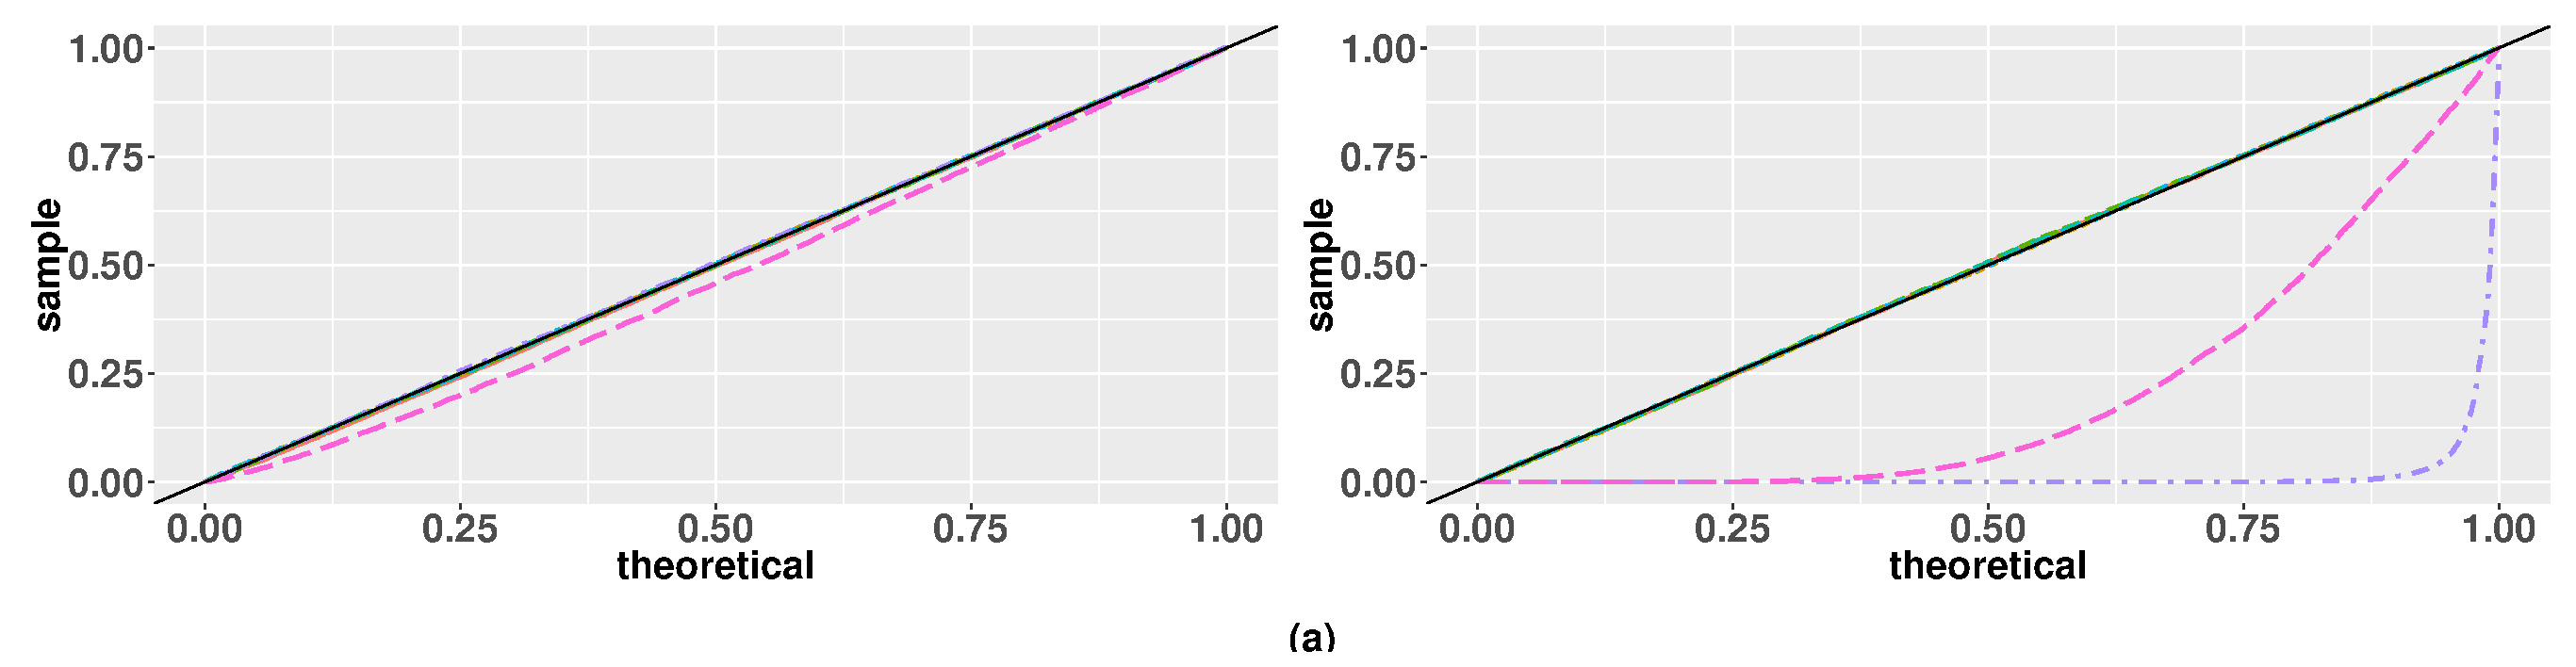
\includegraphics[width=17cm,height=3.9cm]{Figures/parallel_a.eps}
			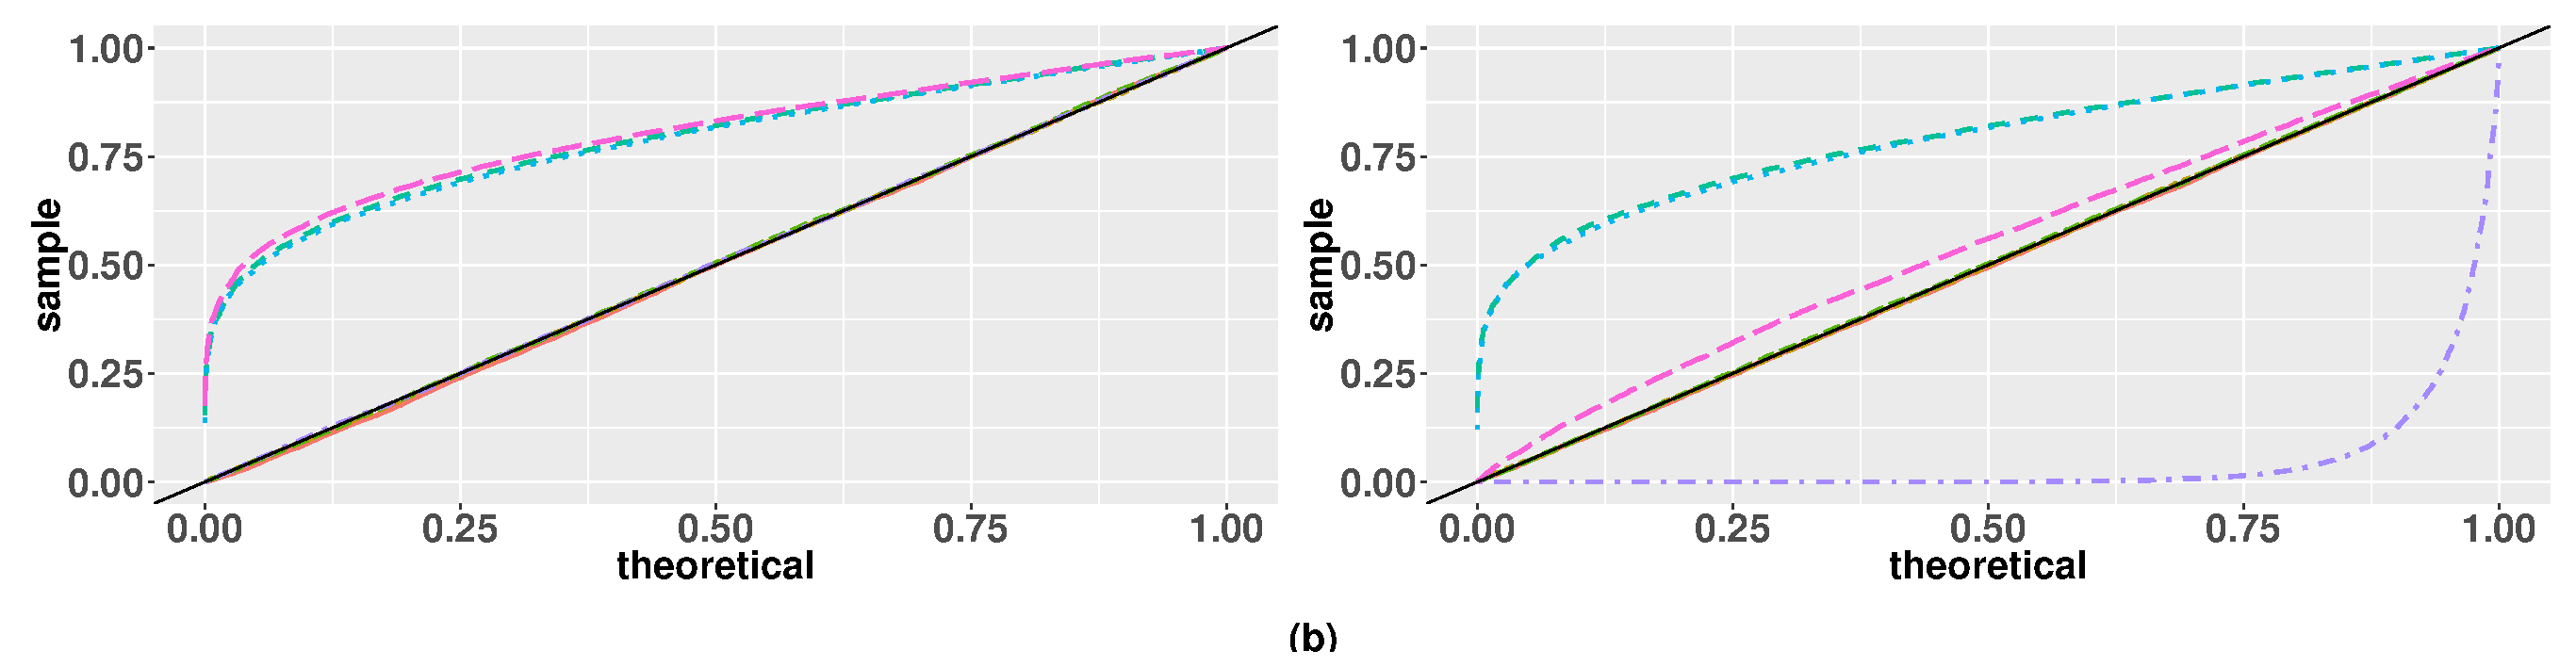
\includegraphics[width=17cm,height=3.9cm]{Figures/parallel_b.eps}
			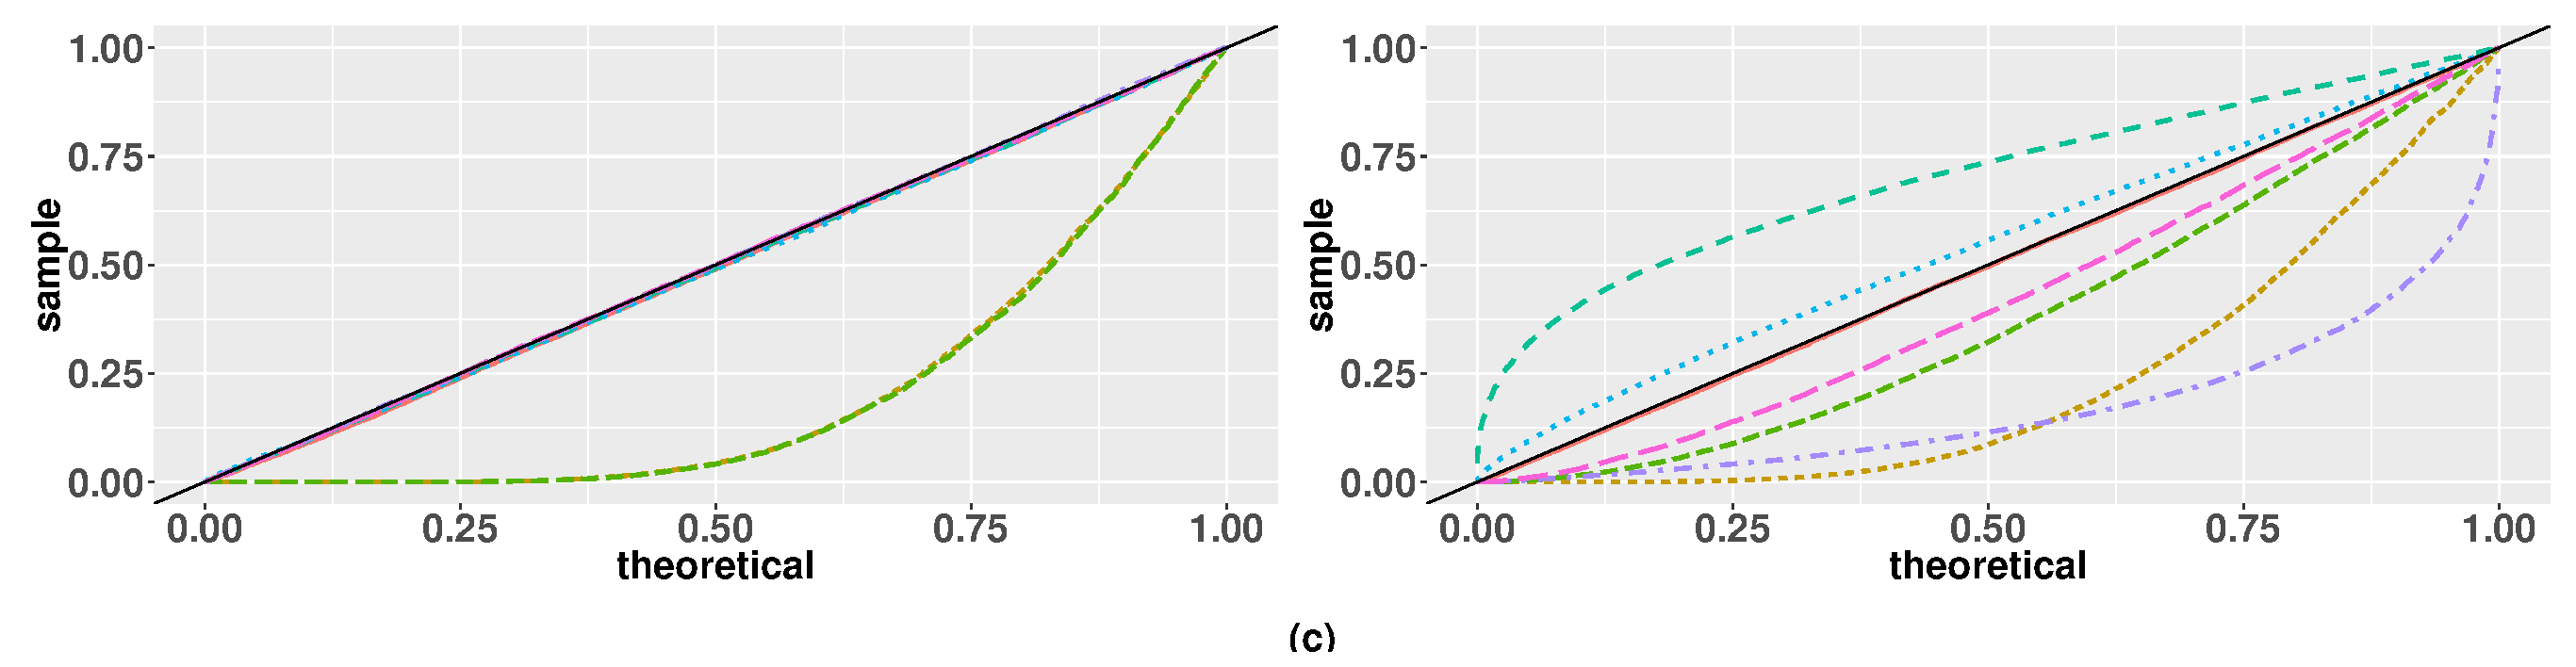
\includegraphics[width=17cm,height=3.9cm]{Figures/parallel_c.eps}
			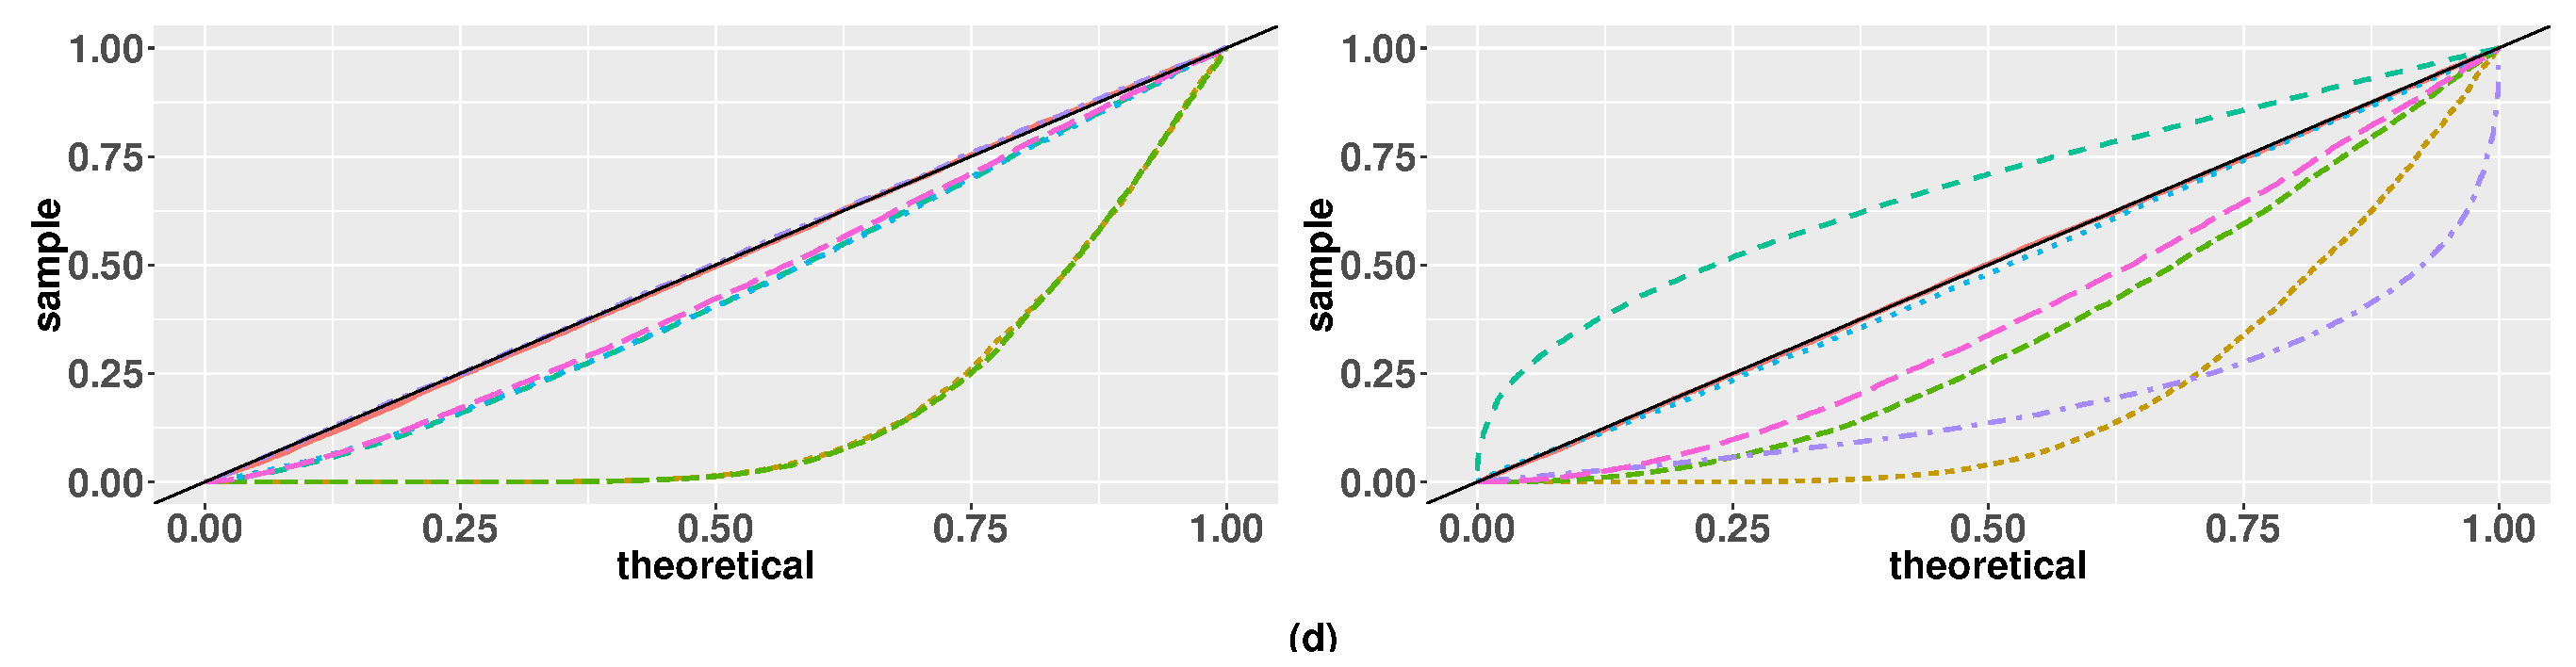
\includegraphics[width=17cm,height=3.9cm]{Figures/parallel_d.eps}
			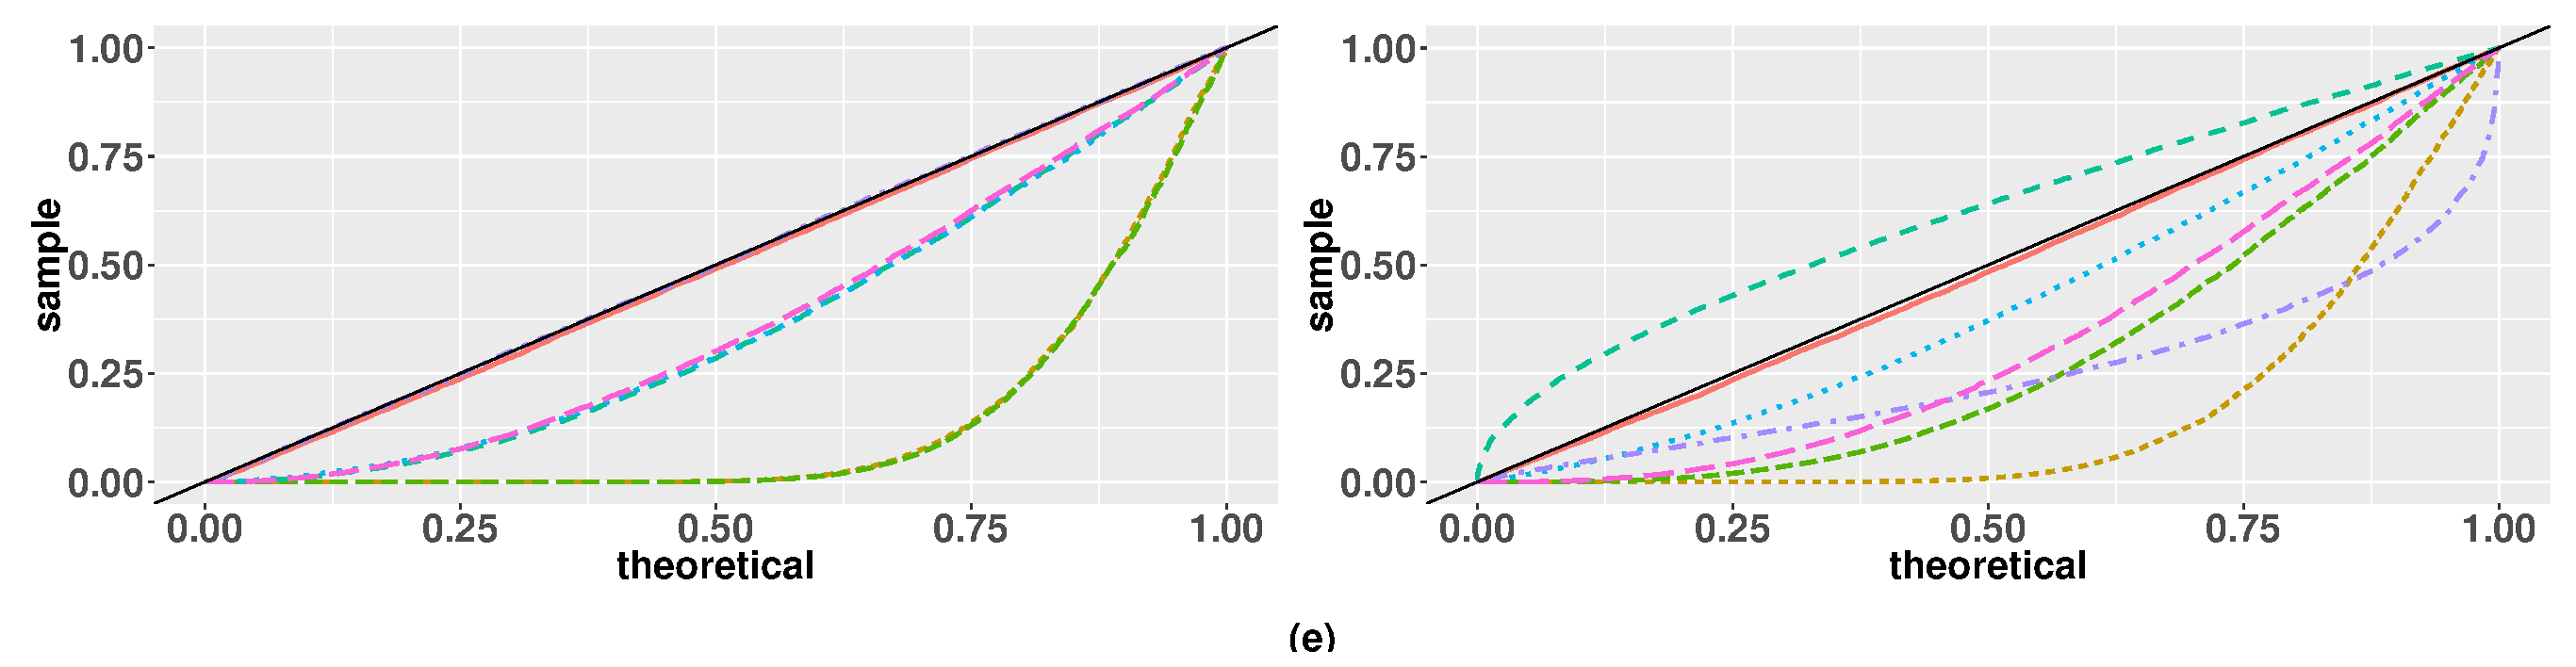
\includegraphics[width=17cm,height=3.9cm]{Figures/parallel_e.eps}
		\end{center} 
		\caption[Uniform quantile-quantile plots for $p$-values by different methods]{Uniform 
			quantile-quantile plots for $p$-values by different methods. Each plot 
			from top to bottom corresponds to correlation structures (\aaCase)-(\fCase), 
			respectively. 
			The left column is for group $A_1$ simulation, and the right column for group $A_2$ 
			simulation (see Table \ref{table:simusetup} for detail). Results are based on
			\HowmanySimu~simulations.}\label{fig:typeIerror}
	\end{figure*} 

	
	\subsection{Power simulation}\label{subsection:power}		 
	
	We compare the power of \OurMethod~to those of the other \HowmanyTest~methods under correlation 
	structure (\aaCase) in which genes are simulated to be independent. 
	Since some of these tests are not well calibrated at the sample size
	considered (see results in Section \ref{subsection:typeIerror}), we report calibrated power. For
	calibrated power, the critical value $c(\alpha)$ is chosen so that when the null hypothesis is 
	true, exactly $100\cdot\alpha\%$ of the resulting $p$-values are less than $c(\alpha)$; that is,
	$c(\alpha)$ is  the $\alpha$ quantile of null distribution of $p$-values, where the null
	distribution is generated from simulation. Calibrated power allows a more fair comparison among
	tests, as tests that are too conservative under the null hypothesis will have greater power due 
	to the tendency to produce small $p$-values, yet this apparent power does not truly distinguish 
	between the null and the alternative.  
	
	Table \ref{table:power} summarizes the calibrated power for the two groups of simulations (i.e.,
	$A_1$ and $A_2$ in Table \ref{table:simusetup}). % We only report the results for correlation
	%structure (\aaCase) where genes are simulated to be independent. %(for power comparisons under 
	%%the
	%other four correlation structures, see online supplementary materials...). %In Table
	%\ref{table:power} we set the DE size $\delta$ to be 0.05 and simulated data in the way that 
	%genes
	%in the background set are not DE (i.e., $p_b=0$). 
	For $A_1$ simulations, GSEA has the highest, and rank based methods (\genr~and \CMR)~have the
	lowest, calibrated power across all four alternative scenarios. \CMT, \gent~and \OurMethod~have 
	no systematic difference in the calibrated power. % Furthermore, when the DE probability is 
	%$10\%$ 
	%or
	%higher (i.e., the case of  $S_2$-$S_4$), both \CMT~and \OurMethod~have comparable calibrated 
	%power
	%to that of GSEA and \gent. In group $A_2$, \gent~continues to achieve the highest calibrated 
	%power
	%while GSEA shows virtually no power. \CMT~and \OurMethod~still have indistinguishable 
	%calibrated
	%power and both are better than \genr and \CMR.
	In group $A_2$ simulations, GSEA shows virtually no power. \OurMethod, \CMT, and \gent~ have
	indistinguishable calibrated power and are among the best.
	%though it is slightly inferior to the best calibrated power from QuSAGE. 
	
	\begin{table*}[!ht]
		\centering
		\caption[Recalibrated power for different methods]{Recalibrated power for different 
			methods under correlation structure (\aaCase) in which genes are simulated to be 
			independent. The $c(\alpha)$ is the $\alpha$ quantile of null distribution of 
			$p$-values. 
			The powers are calculated as the proportion of $p<c(\alpha)$ for each of the four 
			alternatives $S_1$-$S_4$ and each of the group $A_1$ and $A_2$ simulations (see Table 
			\ref{table:simusetup} for detail). Results are based on \HowmanySimu~simulations.
		}\label{table:power}
		%	\begin{tabular}{cl M{2.0cm}M{2.0cm}M{2.0cm}M{2.0cm}M{2.0cm}}
	\begin{tabular}{cp{3cm}p{2cm}p{2cm}p{2cm}p{2cm}p{2cm}}
		\toprule
			Group & Method &$c(\alpha)$	& $S_1$ & $S_2$ & $S_3$	&$S_4$  \\ 
		\colrule
			\multirow{7}{*}{$A_1$} & \OurMethod & 0.045 & 0.340 & 0.741 & 0.944 & 0.991 \\ 
			&	\genr  & 0.051 & 0.111 & 0.284 & 0.533 & 0.766 \\ 
			&	\gent & 0.049 & 0.344 & 0.744 & 0.947 & 0.992 \\ 
			&	\CMT  & 0.051 & 0.336 & 0.737 & 0.943 & 0.990 \\ 
			&	\CMR  & 0.053 & 0.108 & 0.280 & 0.519 & 0.758 \\ 
			&	GSEA & 0.051 & 0.517 & 0.894 & 0.989 & 0.999 \\ 
			&	QuSAGE & 0.028 & 0.385 & 0.784 & 0.959 & 0.995 \\ 
		\colrule
			\multirow{7}{*}{$A_2$} &	MEQLEA & 0.050 & 0.180 & 0.478 & 0.777 & 0.939 \\ 
			&		\genr & 0.048 & 0.104 & 0.269 & 0.530 & 0.781 \\ 
			&		\gent & 0.049 & 0.175 & 0.473 & 0.773 & 0.936 \\  
			&		\CMT & 0.052 & 0.173 & 0.466 & 0.766 & 0.933 \\ 
			&		\CMR & 0.050 & 0.102 & 0.262 & 0.521 & 0.771 \\ 
			&		GSEA & 0.000 & 0.000 & 0.000 & 0.000 & 0.000 \\ 
			&		QuSAGE  & 0.000 & 0.021 & 0.127 & 0.387 & 0.692 \\ 
		\botrule
		\end{tabular}
	\end{table*}
	
	
	
	Figure \ref{fig:power} shows for \OurMethod, the variations in power according to different
	correlation structures across four alternative scenarios $S_1$--$S_4$. For each correlation 
	structure and each alternative, we report the power (without recalibration) at a significance 
	level of 0.05. The top is the power for group $A_1$, and the bottom for group $A_2$.  The 
	powers under correlation structures (\aaCase) and (\cCase) are very similar, and are among the 
	highest under each of the four alternatives. It's not surprising because they correspond to the 
	simplest correlation structures: gene expression values in (\aaCase) are simulated to be 
	independent and in (\cCase) are simulated to have the same correlation 0.1. As the correlation 
	structure becomes more complex, from (\aCase) to (\eCase) then
	to (\fCase), the power decreases under every alternative scenario. The power under correlation
	structure (\fCase) is the lowest for both $A_1$ and $A_2$ simulations.% We also note that the 
	%power
	%decreases when DE genes are present in the background set as compared to the case where there 
	%are
	%no DE genes in the background set. (We might need the same DE size to illustrate this point.)
	
	\begin{figure}[!ht]
		\centering
		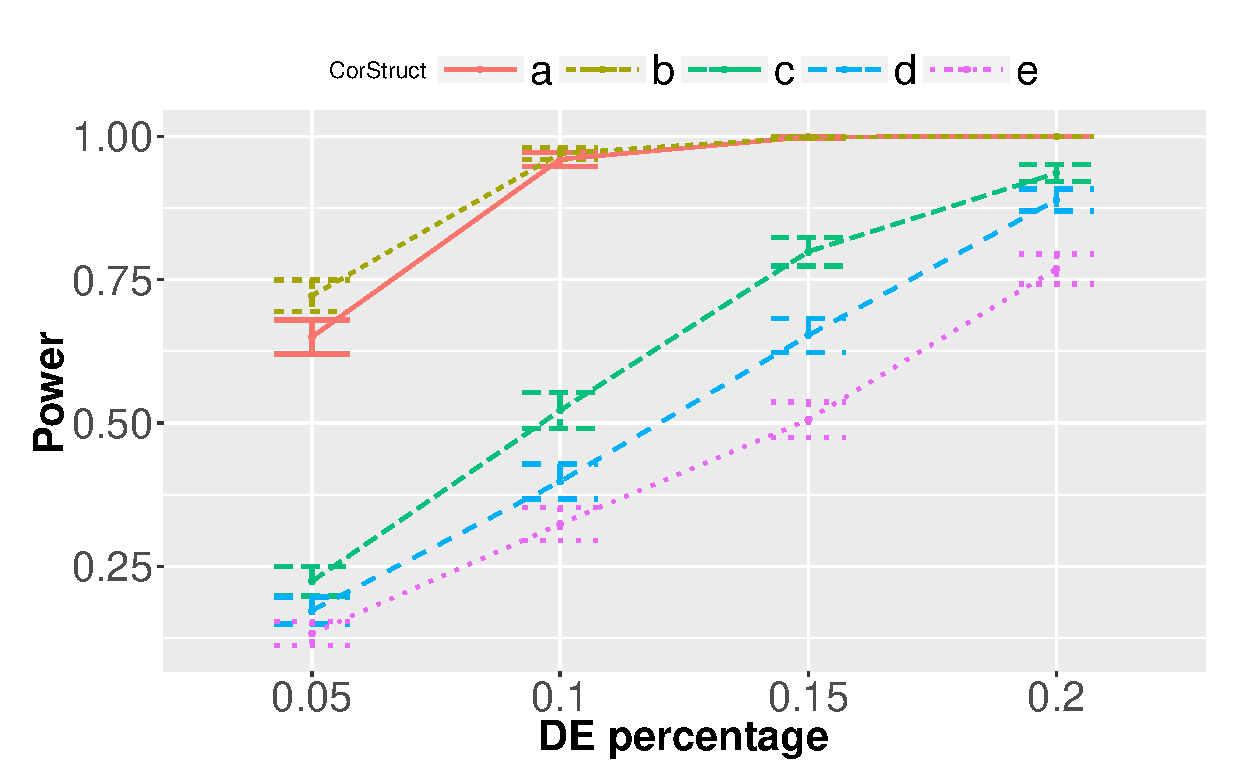
\includegraphics[width=8.5cm,height=5cm]{Figures/powerA1pct.eps}
		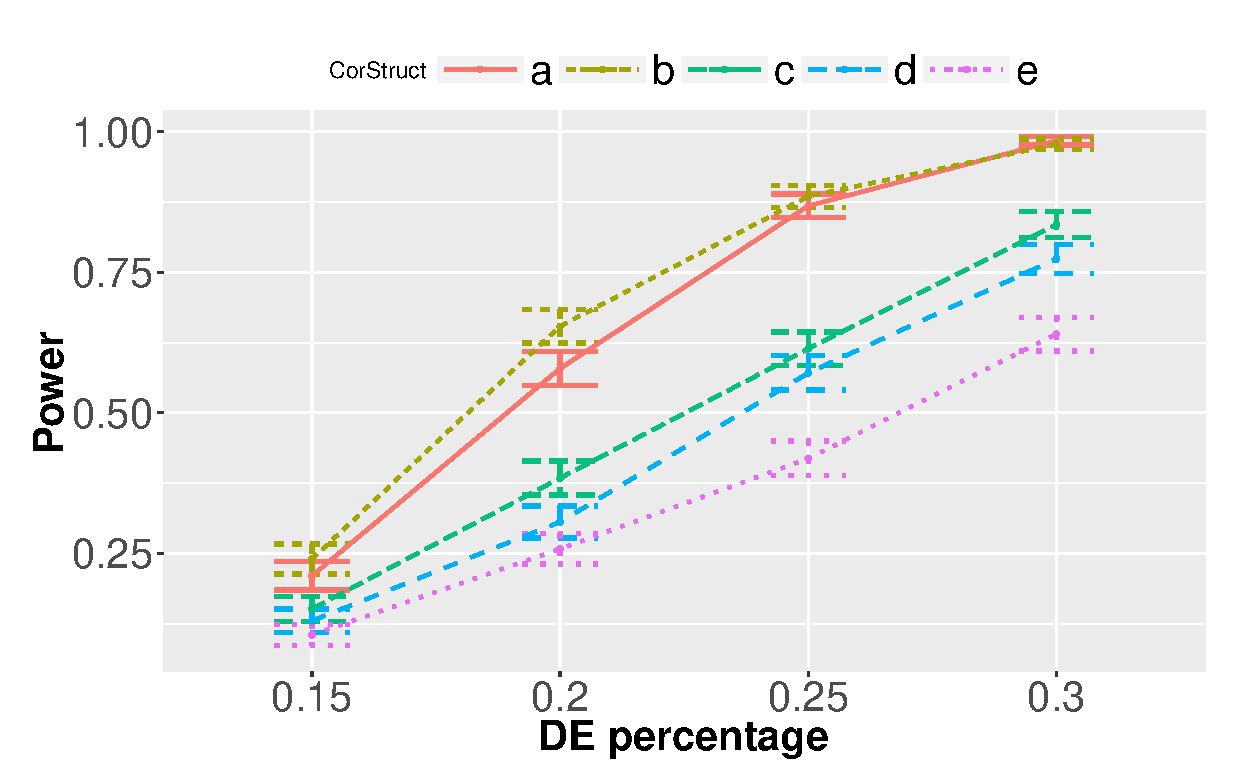
\includegraphics[width=8.5cm,height=5cm]{Figures/powerA2pct.eps}
		\caption[Power for \OurMethod~under correlation structures (\aaCase)-(\fCase)]{Power for 
			\OurMethod~under correlation structures (\aaCase)-(\fCase) of Section
			\ref{subsection:simulation}. The top corresponds to group $A_1$ simulations, and the 
			bottom to group
			$A_2$ simulations (see Table \ref{table:simusetup}). The error bars are the $95\%$ CIs 
			based on
			\HowmanySimu~simulations. }\label{fig:power}
	\end{figure} 

	\subsection{Real Data}\label{section:realdata}
	We apply \OurMethod~to two example data sets, and compare the lists of enriched gene sets to 
	those obtained by other three methods (GSEA, \CMT~and \genr). %In both examples, 
	%\OurMethod~were able 
	%to
	%identify more gene sets as enriched. 
	Our results lend credence to previous studies in finding potential gene sets correlated with
	Huntington's disease and those correlated with chromosome Y and Y bands in lymphoblastoid 
	cells.  
	
	\subsubsection{Huntington's Disease Data}
	We examine the Huntington's Disease (HD) RNA-Sequencing (RNA-Seq) data 
	\citep{labadorf2015rna} to identify enriched gene sets that are potentially responsible for HD. 
	The mRNA expression profiles in human prefrontal cortex were obtained from 20 Huntington's 
	Disease samples and 49 neurologically normal controls.  Expression values are normalized and 
	filtered as described in the methods section of \citet{labadorf2015rna}. The data, containing 
	$28,087$ genes, is available as a series GSE64810 in the GEO database 
	(\url{http://www.ncbi.nlm.nih.gov/geo/}). For each gene, we adjust for two covariates---age at 
	death (DeathAge) and RNA Integrity Number (RIN), as also done by \citet{labadorf2015rna}. We 
	follow their strategy of treating the two covariates as categorical. Briefly, DeathAge is 
	binned into intervals 0-45, 46-60, 61-75, 76-90 and	90+, and RIN is dichotomized as  $>$ (coded 
	as 1) or $\leq$ 7 (coded as 0). We regress the normalized expression levels on AgeDeath and RIN 
	and use the resulting 
	residuals as the \textit{covariate-adjusted expression levels}.
	
	We perform enrichment analysis on the covariate-adjusted data using the MsigDB
	\citep{subramanian2005gene} C2 Canonical Pathways (February 5, 2016, data last accessed).
	The C2 Canonical Pathways have a collection of 1330 gene sets, with an average set size of
	50 (the set sizes range from 3 to 1028, and the median is 29). Since the genes are named by
	HGNC symbols in C2 and by ensembl IDs in the HD expression data set, we convert the ensembl 
	IDs in 	the expression data into HGNC symbols using \textit{BioMart}
	(\url{http://uswest.ensembl.org/biomart/martview/}). We retain $26,941$ genes that have
	corresponding HGNC symbols. 
	
	
	
	We apply four test procedures (\OurMethod, GSEA, \CMT~and \genr) to run enrichment analysis 
	for	the entire C2 Canonical Pathways, and compared the four tests in terms of resulting
	enriched gene sets. %\genr~has been reported to be the best method among four methods that
	%\cite{tarca2013comparison} considered in terms of FDR .
	We use the \FDR~\citep{benjamini1995controlling} procedure (\FDRabb) to control the false
	discovery rate (FDR) for multiple hypothesis testing (unless specified otherwise, all 
	$p$-values in Section \ref{section:realdata} are adjusted by \FDRabb~procedure). The 
	\FDRabb~procedure is used when the test statistics under the null have non-negative 
	correlations \citep{benjamini2001control}. We note that since many pathways have overlapped 
	genes, the \FDRabb~procedure should be appropriate in our study.
	
	In Figure \ref{fig:HDdatap} we plot $-\log 10~p$-values of \OurMethod~against those of GSEA, 
	\CMT~and \genr.
	%Compared to GSEA, smaller $p$-values (e.g., less than 0.1) resulting from \OurMethod~are more 
	%likely
	%to cluster---in contrast to larger $p$-values; that is, \OurMethod~produces more small 
	%$p$-values
	%than GSEA does while \OurMethod~and GSEA do not differ much in producing larger $p$-values. 
	The $p$-values of \CMT~are overwhelmingly larger than their counterparts of GSEA or \OurMethod, 
	yet smaller than those of \genr, even 
	if $p$-values between \OurMethod~and other three methods are highly correlated (Pearson's 
	correlation of $\log 10 ~p$ between \OurMethod~and GSEA, \CMT~and \genr~are 0.90, 0.96, and 
	0.87 respectively). This trend of $p$-values is consistent with our earlier simulation (see 
	results in simulation section \ref{subsection:typeIerror}) that
	\CMT~could produce large $p$ values. The $p$-values of \genr~are in general smaller than the 
	corresponding $p$-values of \OurMethod, leading to more significant calls. 
		
		\begin{figure}[h!]
			\begin{center}
				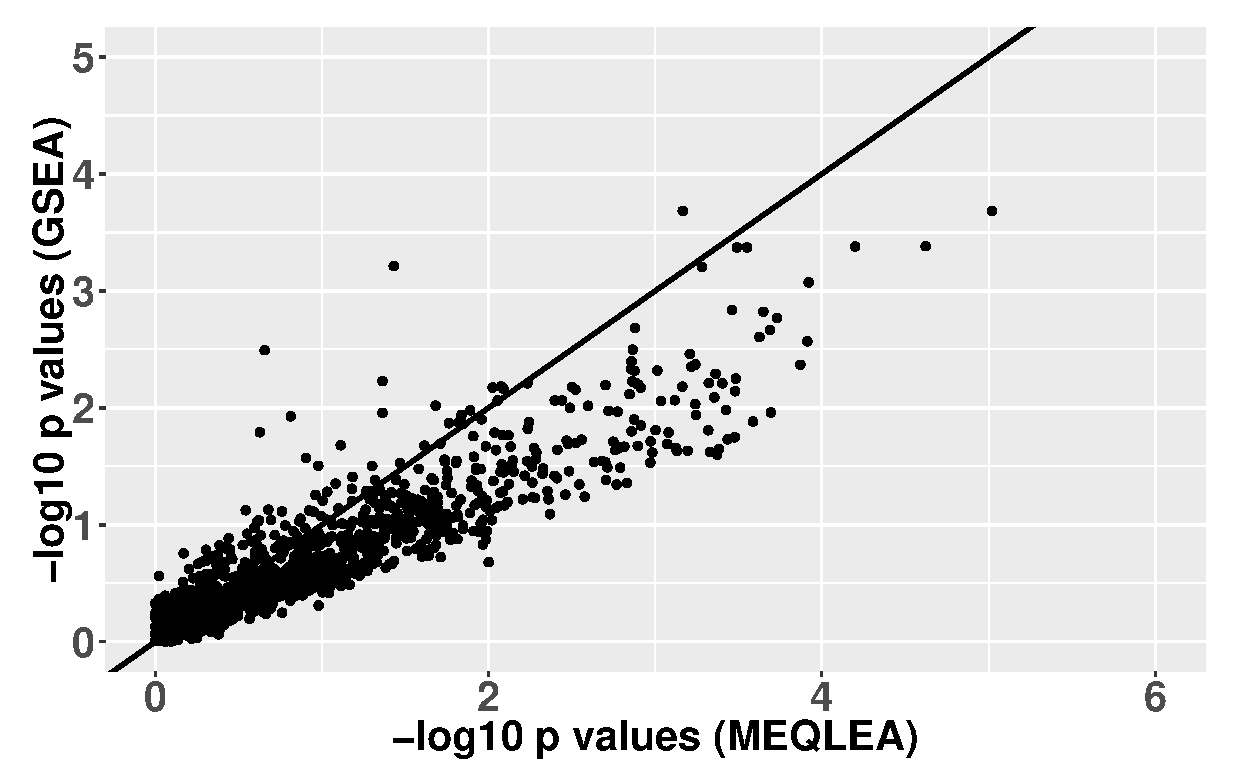
\includegraphics[width=8cm,height=5cm]{Figures/MEQLEA_GSEA.eps}
				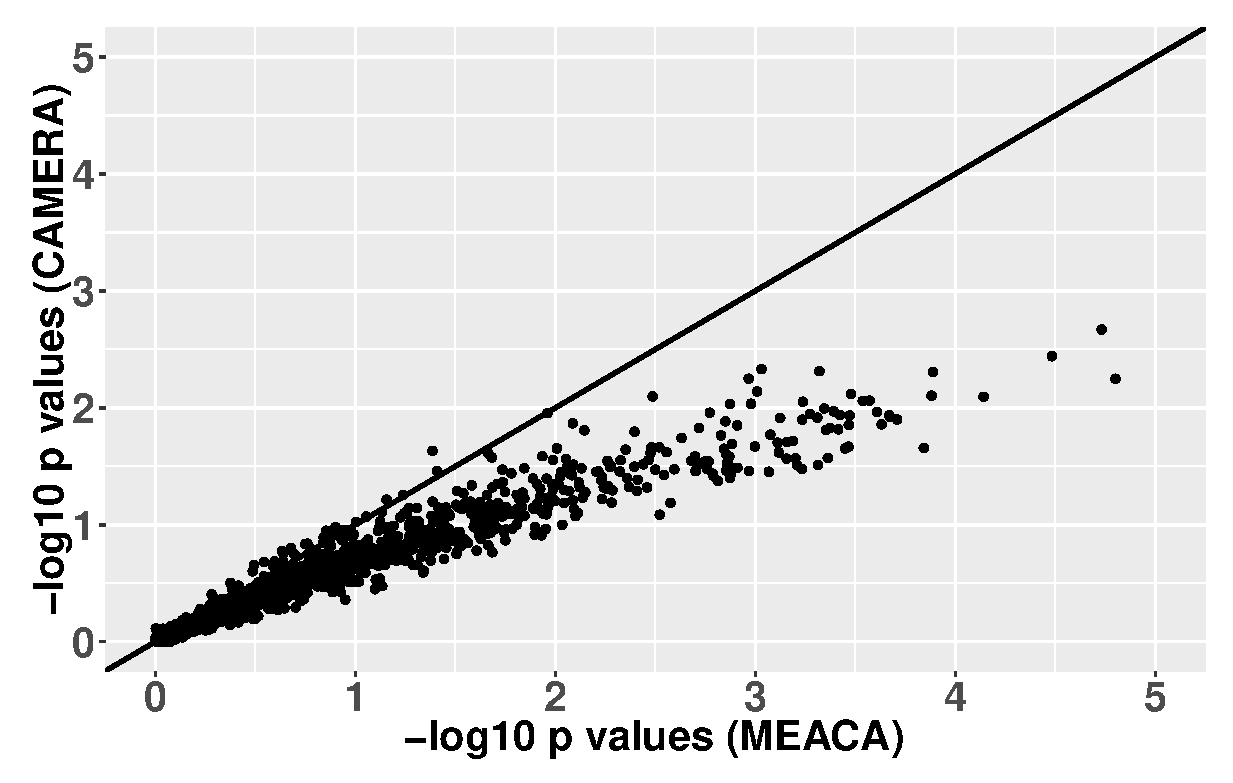
\includegraphics[width=8cm,height=5cm]{Figures/MEQLEA_Camera.eps}
				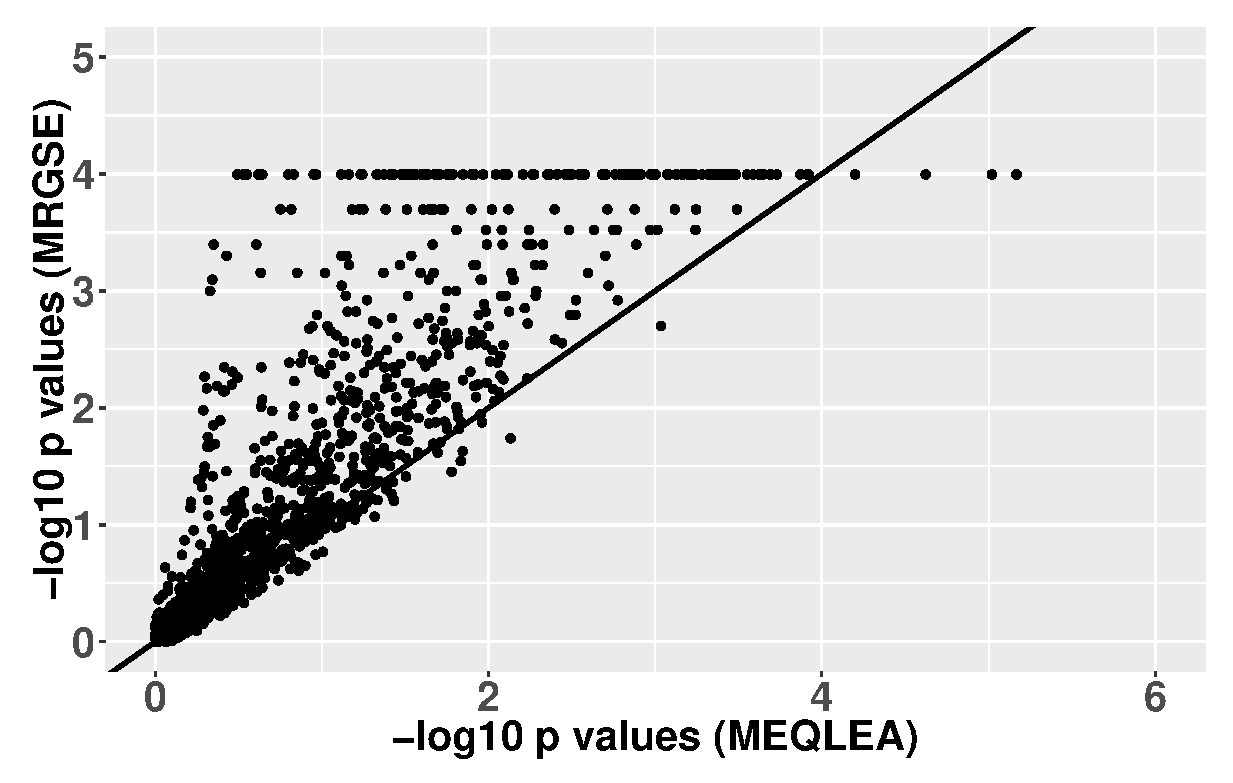
\includegraphics[width=8cm,height=5cm]{Figures/MEQLEA_MRGSE.eps}
			\end{center} 
			\caption[Pairwise comparisons of $p$-values for different methods]{Pairwise comparisons 
			of $p$-values for \OurMethod, GSEA, \CMT and \genr. The $p$-values 
				are reported from enrichment test of each gene set in the C2 Canonical Pathway gene 
				sets.
			}\label{fig:HDdatap}
		\end{figure} 
		
		%	\begin{figure}
		%		\begin{center}
		%			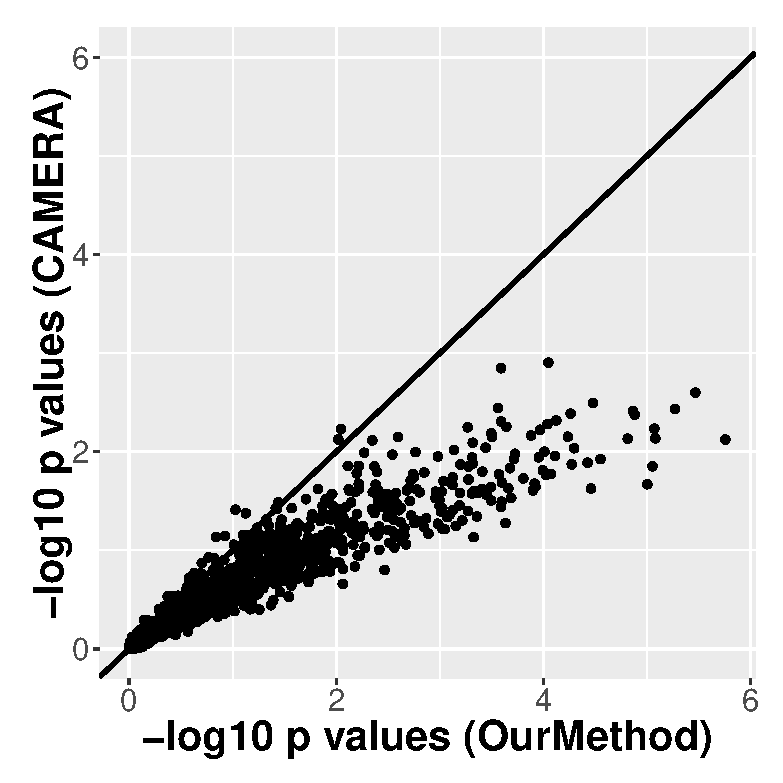
\includegraphics[width=5.5cm,height=5cm]{Figures/log10P_Camera.eps}
		%			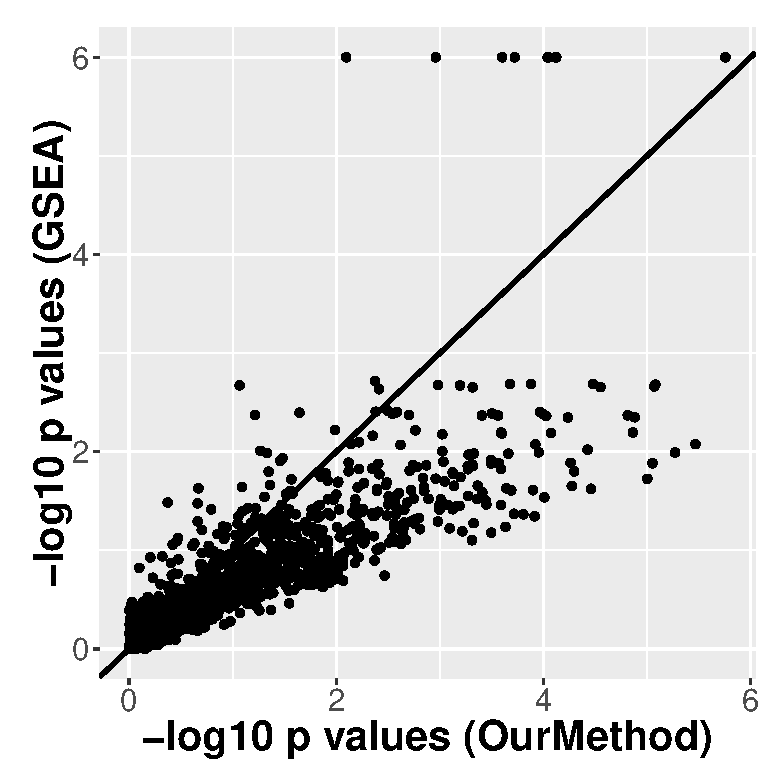
\includegraphics[width=5.5cm,height=5cm]{Figures/log10P_GSEA.eps}
		%			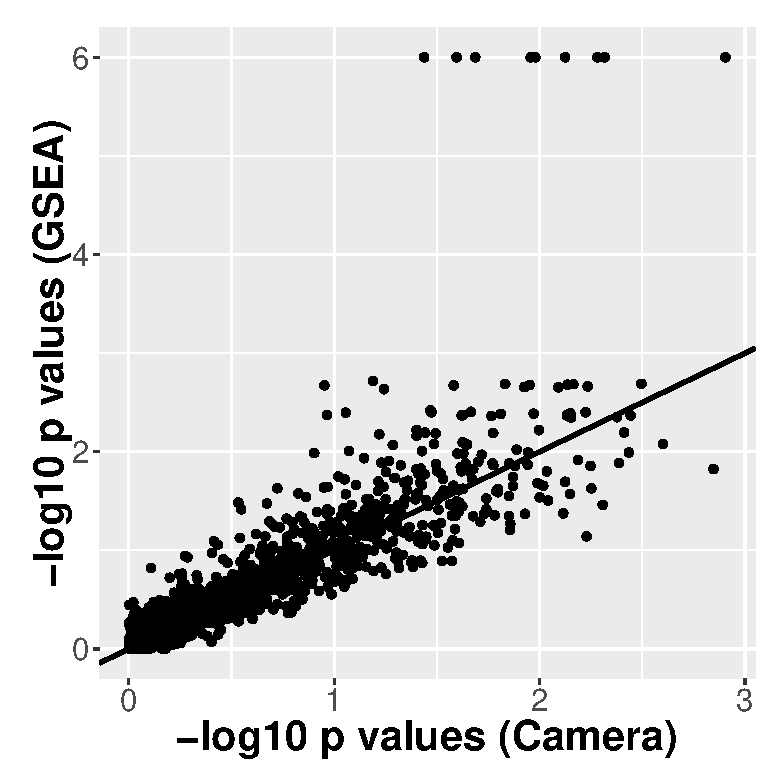
\includegraphics[width=5.5cm,height=5cm]{Figures/log10P_GSEA_CAMERA.eps}
		%		\end{center} 
		%				\caption{raw p value plots for different methods, -log10(p  + 
		%1e-6)}\label{fig:HDdatalog10p}
		%	\end{figure} 
		
	Using \OurMethod, we find 89 significant signals out of the entire 1330 gene sets at FDR level
	of 0.05. GSEA finds 3 enriched gene sets---2 of them were also among those 89 gene sets (the one
	that is not significant according to \OurMethod~had a $p$-value of 0.013 and FDR 0.100).
	\genr~identified 387 gene sets which include all the 89 sets \OurMethod~identified, and 
	\CMT~identified none. Originally, \citet{labadorf2015rna} used the same HD data set to conduct 
	enrichment analysis using topGo \citep{alexa2010topgo}. They note that the enriched gene sets 
	they identified show a clear immune response and inflammation-related pattern, including 
	``REACTOME INNATE IMMUNE SYSTEM," ``PID IL4
	2PATHWAY," and ``PID NFKAPPAB CANONICAL PATHWAY". These three gene sets rank (by nominal
	$p$-values) 18, 10 and 3 respectively in the 89 enriched gene sets.
	
	In Table \ref{table:top30}, we report the top 30 enriched gene sets (ordered by nominal $p$ 
	values) identified using \OurMethod. We also label the enriched gene sets from GSEA by 
	``$\ast$" in the table. Many of our enriched gene sets have been shown to be closely related to 
	HD pathogenesis. For example, the top enriched gene set by \OurMethod, ``PID SMAD2 3NUCLEAR 
	PATHWAY," is responsible for regulation of nuclear SMAD2/3 signaling. 
	\citet{katsuno2010disrupted} showed that nuclear SMAD2/3 are
	related to polyglutamine disease, which includes HD. The third enriched gene set, ``PID NFKAPPAB
	CANONICAL PATHWAY," is a canonical NF-kappaB pathway, and its dysregulation causes HD immune
	dysfunction \citep{trager2014htt}. Also, \citet{marcora2010huntington} found that reduced 
	transport of NF-kappaB out of dendritic spines and its activity in neuronal nuclei may 
	contribute to the etiology of HD. 
	%HD mutation can reduce the transport of NF-kappaB out of dendritic spines and its activity in
	%neuronal nuclei and this reduction may contribute to the etiology of HD. 
	Another gene set, ``REACTOME INNATE IMMUNE SYSTEM," contributes to HD pathogenesis
	\citep{labadorf2015rna,trager2014htt}. %\cite{diamanti2013whole} showed that ``REACTOME
	% TRANSCRIPTIONAL ACTIVITY OF SMAD2 SMAD3 SMAD4 HETEROTRIMER," a gene set involved in 
	%transcriptional
	%activity of SMAD2/SMAD3:SMAD4 heterotrimer, is also enriched in their microarray study of HD
	%pathology from blood samples of R6/2 at manifest stage and wild type littermate mice. 
	%For AKT signaling pathway, ``BIOCARTA AKT PATHWAY," \cite{humbert2002igf} demonstrated that
	%huntingtin is a substrate of AKT and that phosphorylation of huntingtin by AKT is crucial to 
	%mediate
	%the neuroprotective effects of IGF-1. They also showed that AKT is altered in Huntington?s 
	%disease patients.  
	\citet{chiang2010modulation} demonstrated that the systematic downregulation of PPAR$\gamma$,
	related to ``BIOCARTA PPARA PATHWAY," seems to play a critical role in the dysregulation of 
	energy homeostasis observed in HD, and that PPAR$\gamma$ is a potential therapeutic target for 
	this disease. %For ``REACTOME SIGNALING BY TGF BETA RECEPTOR COMPLEX,"  
	%\cite{kandasamy2011transforming}
	%demonstrated that TGF-beta1 signaling appears to be a crucial modulator of neurogenesis in HD
	%pathology and it can be a promising target for endogenous cell-based regenerative therapy. 
	For ``PID P53 DOWNSTREAM PATHWAY," \citet{ghose2011regulation} showed the likely involvement of 
	NFkB (RelA), p53 and miRNAs in the regulation of cell death in HD pathogenesis. 
	
		
		\begin{table*}[!ht]
			%	\label{table:gender} 
			\centering 
	\caption[Enriched gene sets (ordered by nomial $p$-values) identified by \OurMethod~for HD 
	data]{Enriched gene sets (ordered by nomial $p$-values) identified by \OurMethod~for HD 
		data. The $\hat\rho_1$,  $\hat\rho_2$ and $\hat\rho_3$, respectively, are the average 
		estimated sample correlations of observed data between genes in the test set, between genes 
		in the background set, and between cross-category genes. The enriched gene sets are noted 
		by ``$\ast$" for GSEA. No gene set was identified as enriched by \CMT~and all the 30 gene 
		sets are also identified as enriched by \genr. For all methods, a gene set is called 
		significant when its FDR using \FDR~(\FDRabb) correction is $<0.05$. }
			%	\begin{tabular}{p{3in}M{0.5cm}M{0.7cm}M{0.7cm}M{0.7cm}M{1.5cm}M{1.5cm}M{0.8cm}} 
			
		\begin{tabular}{p{3in}rrrrrrr}
			\toprule
			Gene Set & Size & $\hat\rho_1$ & $\hat\rho_2$ & $\hat\rho_3$ & $p$-value & FDR & \\ 
			\colrule
			PID SMAD2 3NUCLEAR PATHWAY & 79 & 0.063 & 0.013 & 0.015 & 5.8E-06 & 5.7E-03 & $\ast$ \\ 
			REACTOME YAP1 AND WWTR1 TAZ STIMULATED GENE EXPRESSION & 23 & 0.121 & 0.013 & 0.014 & 
			8.5E-06 & 5.7E-03 &  \\ 
			PID NFKAPPAB CANONICAL PATHWAY & 22 & 0.127 & 0.013 & 0.019 & 2.3E-05 & 1.0E-02 &  \\ 
			BIOCARTA NTHI PATHWAY & 23 & 0.130 & 0.013 & 0.023 & 6.2E-05 & 2.1E-02 &  \\ 
			BIOCARTA TID PATHWAY & 18 & 0.101 & 0.013 & 0.012 & 1.2E-04 & 2.2E-02 &  \\ 
			PID HIV NEF PATHWAY & 35 & 0.065 & 0.013 & 0.013 & 1.2E-04 & 2.2E-02 &  \\ 
			KEGG PATHWAYS IN CANCER & 311 & 0.028 & 0.013 & 0.010 & 1.3E-04 & 2.2E-02 &  \\ 
			PID MYC REPRESS PATHWAY & 60 & 0.057 & 0.013 & 0.013 & 1.9E-04 & 2.2E-02 &  \\ 
			BIOCARTA TOLL PATHWAY & 36 & 0.083 & 0.013 & 0.018 & 2.0E-04 & 2.2E-02 &  \\ 
			PID IL4 2PATHWAY & 59 & 0.081 & 0.013 & 0.010 & 2.0E-04 & 2.2E-02 &  \\ 
			KEGG TGF BETA SIGNALING PATHWAY & 82 & 0.055 & 0.013 & 0.011 & 2.2E-04 & 2.2E-02 &  \\ 
			BIOCARTA DEATH PATHWAY & 33 & 0.067 & 0.013 & 0.013 & 2.4E-04 & 2.2E-02 &  \\ 
			KEGG NOD LIKE RECEPTOR SIGNALING PATHWAY & 55 & 0.045 & 0.013 & 0.008 & 2.6E-04 & 
			2.2E-02 &  \\ 
			BIOCARTA CTCF PATHWAY & 23 & 0.083 & 0.013 & 0.015 & 2.8E-04 & 2.2E-02 &  \\ 
			ST TUMOR NECROSIS FACTOR PATHWAY & 28 & 0.031 & 0.013 & 0.014 & 3.2E-04 & 2.2E-02 &  \\ 
			BIOCARTA TNFR2 PATHWAY & 17 & 0.151 & 0.013 & 0.022 & 3.3E-04 & 2.2E-02 &  \\ 
			KEGG APOPTOSIS & 82 & 0.036 & 0.013 & 0.008 & 3.3E-04 & 2.2E-02 &  \\ 
			REACTOME INNATE IMMUNE SYSTEM & 209 & 0.039 & 0.013 & 0.009 & 3.3E-04 & 2.2E-02 &  \\ 
			PID HES HEY PATHWAY & 47 & 0.071 & 0.013 & 0.019 & 3.4E-04 & 2.2E-02 &  \\ 
			REACTOME DOWNSTREAM TCR SIGNALING & 31 & 0.082 & 0.013 & 0.011 & 3.7E-04 & 2.2E-02 &  
			\\ 
			PID TCPTP PATHWAY & 42 & 0.076 & 0.013 & 0.010 & 3.7E-04 & 2.2E-02 &  \\ 
			BIOCARTA 41BB PATHWAY & 14 & 0.110 & 0.013 & 0.023 & 3.9E-04 & 2.2E-02 &  \\ 
			PID FRA PATHWAY & 34 & 0.154 & 0.013 & 0.008 & 4.1E-04 & 2.2E-02 &  \\ 
			PID P53 DOWNSTREAM PATHWAY & 131 & 0.045 & 0.013 & 0.012 & 4.2E-04 & 2.2E-02 &  \\ 
			PID EPO PATHWAY & 34 & 0.069 & 0.013 & 0.013 & 4.3E-04 & 2.2E-02 &  \\ 
			BIOCARTA PPARA PATHWAY & 53 & 0.031 & 0.013 & 0.008 & 4.4E-04 & 2.2E-02 &  \\ 
			BIOCARTA EPONFKB PATHWAY & 11 & 0.068 & 0.013 & 0.010 & 4.7E-04 & 2.2E-02 &  \\ 
			BIOCARTA HIVNEF PATHWAY & 58 & 0.063 & 0.013 & 0.019 & 4.8E-04 & 2.2E-02 &  \\ 
			BIOCARTA CD40 PATHWAY & 13 & 0.165 & 0.013 & 0.026 & 4.8E-04 & 2.2E-02 &  \\ 
			BIOCARTA IL7 PATHWAY & 17 & 0.100 & 0.013 & 0.016 & 5.2E-04 & 2.3E-02 &  \\ 
			\botrule
			%	\hline\hline
		\end{tabular}
			\label{table:top30}
		\end{table*}
		
		
		
		%	
	%	
	
	
\subsubsection{Male vs Female Lymphoblastoid Cells Data}
	We analyze the mRNA expression profiles from lymphoblastoid cell lines derived from 17 females 
	and	15 males. \citet{subramanian2005gene} examined this data set with their GSEA method, 
	testing the enrichment of the  cytogenetic gene sets (C1). The C1 includes 24 sets, one for 
	each of the 24 human chromosomes, and 295 sets corresponding to cytogenetic bands. For the 
	comparison ``\text{male} VS \text{female}," they expected to find gene sets on chromosome Y, 
	not on chromosome X. We run enrichment analysis with the four tests (\OurMethod, GSEA,\CMT and 
	\genr). In Table \ref{table:gender}, we summarize all the gene sets that are called significant 
	at FDR level $0.05$ by at least one of the four test procedures. Unanimously, three gene 
	sets---``chrY," ``chrYq11" and ``chrYp11"---are 
	found to be enriched by all of the four methods. It is interesting to note that only 
	\OurMethod~is able to identify another Y band, ``chrYp22," as enriched. In fact, these four 
	gene sets are the only four pathways containing at least 3 genes in  C1 and corresponding to 
	chromosome Y or Y bands. \OurMethod~does not produce small $p$-value ($<0.01$) for the 
	remaining three gene sets in Table \ref{table:gender}, which is just as expected in that study.
	
	\begin{table*}[!ht]
		%	\label{table:gender} 
		\centering
		\caption[Enriched gene sets and their nominal $p$ values for lymphoblastoid cells 
		data]{Enriched gene sets and their nominal $p$ values for lymphoblastoid cells data. 
			Reported are gene sets with $\text{FDR}<0.05$ for at least one of the \OurMethod, GSEA, 
			\CMT~and \genr~methods using \FDR~(\FDRabb) procedure.}
	\begin{tabular}{p{3cm}p{1cm}p{3cm}p{2cm}p{3cm}p{2cm}p{2cm}} \toprule
	%	\begin{tabular}{lrrrrr} \toprule
			Gene set & Size & \OurMethod & GSEA & \CMT & \genr \\ 		\colrule
			chrY & 40 & 0.0E+00 & 0.0E+00 & 1.0E-05 & 5.9E-07 \\ 
			chrYq11 & 16 & 0.0E+00 & 0.0E+00 & 7.2E-08 & 8.5E-06 \\ 
			chrYp11 & 18 & 2.1E-15 & 0.0E+00 & 2.8E-04 & 5.1E-04 \\ 
			chrYp22 & 8 & 3.6E-04 & 1.2E-02 & 1.0E-02 & 1.3E-02 \\ 
			chr6 & 614 & 5.6E-02 & 6.0E-01 & 6.1E-01 & 2.1E-04 \\ 
			chr1 & 1104 & 6.1E-02 & 5.5E-01 & 6.3E-01 & 5.3E-05 \\ 
			chr12 & 571 & 8.7E-02 & 2.6E-01 & 4.0E-01 & 5.1E-09 \\ 
			\botrule
		\end{tabular}
		\label{table:gender}
	\end{table*}
	
	\section{Conclusion and Discussion}\label{section:conclusion}
	
		% Conclusion
	 \OurMethod~is a mixed-effects quasi-likelihood model for competitive gene-set 
	 test. It effectively adjusts for completely unknown, unstructured correlations among the 
	 genes. It uses a score test approach and allows for analytical assessment of $p$-values. 
	 Compared to existing approaches, \OurMethod~controls type I error correctly and maintains good 
	 power under different correlation structures.  
	 
	 % What we propose
	 Under the competitive gene-set test framework, a number of methods have been
	 proposed to account for correlation among genes. One approach is to evaluate the set-level 
	 statistic by permuting sample labels to generate the null distribution, as adopted by the 
	 widely used procedure GSEA \citep{subramanian2005gene}. However, sample permutation method has 
	 been criticized for altering the null hypotheses being tested 
	 \citep{goeman2007analyzing,khatri2012ten}. Instead, CAMERA \citep{wu2012camera} proposed to 
	 correct for the correlations among genes by estimating a VIF directly from the data. 
	 Incorporating VIF into set-level test statistics has also been used by 
	 \citet{yaari2013quantitative} in their QuSAGE procedure where 
	 they quantify the gene	 set activity by a probability density function. The 
	 problems with this VIF approach are that it does not properly model the heterogeneity among 
	 genes in terms of the presence and magnitude of DE effect, and that it is intended to account 
	 for test-statistic correlations but is estimated from sample correlations of observed data. We 
	 have argued (in Chapter \ref{chap2}) that the correlations among gene-level statistics may not 
	 be approximated by the sample correlation of observed data due to the presence of \DED~genes. 
	 Such problems will undermine the performances of CAMERA and QuSAGE. In contrast, 
	 \OurMethod~models the covariance of gene-level statistics by two variance components, one 
	 attributable to correlations among samples after treatment effect 
	 removed, and the other attributable to the heterogeneity of DE effects. We note that for	
	 \OurMethod, the estimation of covariance among gene-level statistics need not be exact:
	 \OurMethod~uses a score test that involves linear combinations of the entries of the covariance
	 matrix. The denominator in the score test statistic (see equation (\ref{eq:meqleastat})) can 
	 usually be accurately approximated given the high dimensionality of the covariance matrix. 
	 \OurMethod~is based on quasi-likelihood, therefore it does not require normal assumption of 
	 expression data, and could be applied to both microarray and RNA-Seq experiments. 
	 
	 %(Summarize the results) 
	 We compare the performance of \OurMethod~to those of other existing approaches through both 
	 simulation study and real data analyses. In the simulation study, we examine the calibration 
	 of \OurMethod~and other six method (\gent, \genr, \CMT, \CMR, GSEA and QuSAGE) in terms of 
	 type I error control and power. We demonstrate that \OurMethod~holds correct type I error size 
	 under all correlation structures considered, whereas all other methods may fail in one or more 
	 situations. \OurMethod~is also among the best in terms of power performance even under 
	 independent correlation structure. In the real data analyses, we run enrichment analysis using 
	 four methods---\OurMethod, \CMT, GSEA and \genr---on two data sets.
	 The $p$-values of \OurMethod~are smaller than those produced by 
	 GSEA and CAMERA that are intended to adjust for between-gene correlations, but 
	 larger than those of \genr~that assumes independence between genes.
	 \OurMethod~is able to identify a moderate size of enriched gene sets, many of which are 
	 confirmed by independent studies yet are not revealed by other three methods.
	 
	 Currently, \OurMethod~only supports enrichment test for two-group comparisons. In
	 many gene expression experiments, however, researchers might use more complex design to study
	 different factors of interest, in which case a (generalized) linear model would be more 
	 appropriate. Our future work will focus on generalizing \OurMethod~to allow for more 
	 complicated design structures. 
	 
	 The R codes for reproducing results in this paper are available at
	 \url{https://github.com/zhuob/EnrichmentAnalysis}.
		%Using the terminology of \cite{khatri2012ten}, these methods generally fall into three 
		%categories:
		%\textit{over-representation analysis}, \textit{functional class scoring} and 
		%\textit{pathway
		%topology}. The over-representation analysis evaluates a fraction of genes among a set of
		%pre-selected interesting genes (e.g., differentially expressed genes between treatment 
		%versus
		%control samples). The test is usually conducted in the form of $2\times 2$ table, for 
		%example,
		%GOstat of \cite{klebanov2007multivariate} and GO:TermFinder of \cite{tian2005discovering}. 
		%However,
		%the over-representation analysis methods have inherent limitations such as information 
		%loss by
		%choosing arbitrary threshold (e.g., $p$-value $< 0.05$), or problematic assumption of 
		%independence
		%of genes \citep{goeman2007analyzing, wu2012camera}. The functional class scoring performs
		%three-stage analysis \citep{khatri2012ten}: on the first stage, a \textit{gene-level 
		%statistic}
		%that measures the association between the expression levels and the experimental design 
		%variables
		%is calculated for each gene; such gene-level statistics include, among others, 
		%signal-to-noise
		%ration \citep{subramanian2005gene}, moderated $t$ statistics \citep{Smyth2004moderated} 
		%and 
		%$Z$-score \citep{efron2007correlation}. On the second stage, a \textit{set-level 
		%statistic} is
		%calculated by using gene-level statistics and prior information about the test set (i.e., 
		%whether
		%the gene belongs to the set) as input. On the last stage, a $p$-value is assigned to the 
		%test 
		%set
		%by comparing the set-level statistic to its reference distribution.  (Rewrite this part)	
		%The
		%pathway topology will not be discussed in this paper 
		%\citep{khatri2012ten,tarca2013comparison}.
		
		%\section{Conclusion}\label{section:conclusion}
		
	
	
	
	
	\section{Acknowledgments}\label{section:acknowledgment}
	
	The work of BZ in this article was partially supported by the National Institute of 
	General Medical Sciences of the National Institutes of Health under Award Number R01GM104977 
	(to YD, SCE, and JHC). We thank Yanming Di, Sarah Emerson and Wanli Zhang for helpful 
	discussion in preparing this manuscript. We thank Dr. Adam Labadorf for providing information 
	about the HD gene expression data. %This article is part of doctor dissertation written by BZ 
	%under the supervision of YD.

	
	
	\subsubsection{Conflict of interest statement.} None declared.
	
	\newpage
	
		\section*{Appendix}\label{section:appendix}
		
		
	\subsection{Standardization}\label{app:standardization} 
	Standardization for each gene: first, we obtain the residuals by subtracting off the means 
	within 
	each treatment group;
	\begin{equation}
		r_{ijk} = y_{ijk} - \sum_{j=1}^{n_k}{y}_{ijk}/n_k;
	\end{equation}
	then we calculate the pooled standard deviation from the residuals,
	\begin{equation}
		s_i = \textit{std}(r_{ijk});
	\end{equation}
	next we get the standardized expression by dividing the original expression levels by the
	standard deviation,
	\begin{equation}
		y^{\ast}_{ijk} = y_{ijk}/s_i
	\end{equation}
	We perform the standardization procedure to every gene in the data set.\\
	
	\subsection{Covariance matrix for test statistics}\label{app:covariance}
	Note that if we let $\delta_i$ be the DE size for gene $i$, then $E(\delta_i)= \mu_{\delta}$ 
	and $\var(\delta_i) = \sigma_{\delta}^2$. To prove the equation (\ref{eq:DeltaBinom}), we 
	introduce an additional random variable $Z_i$ for DE status, where 
	$Z_i\sim \text{Bernoulli}(1, p_t)$ if $G_i = 1$ and $Z_i\sim \text{Bernoulli}(1, p_b)$ if $G_i 
	= 0$. It follows that $\Delta_i =Z_i\delta_i$, and we have 
	\begin{equation}\notag
		E(\Delta_i|\bm G) = E(Z_i\delta_i|\bm G) = E(\delta_i)E(Z_i|\bm G)=  p_i\mu_{\delta},
	\end{equation}
	and 
	\begin{equation}\notag
		\begin{aligned}
			\text{Var}(\Delta_i|\bm G) & = E[(Z_i\delta_i)^2|\bm G]- [E(Z_i\delta_i|\bm G)]^2 \\
			& = \text{Var}(Z_i|\bm G)[E(\delta_i)]^2 + \left[(EZ_i|\bm G)^2 + 
			\text{Var}(Z_i|\bm G)\right]\text{Var}(\delta_i) \\
			& =p_i\sigma_{\delta}^2 + p_i(1-p_i)\mu_{\delta}^2.
		\end{aligned}
	\end{equation}
	If the gene-level test statistics $U_i$'s take the form of equation (\ref{eq:U}), then we have 
	$E(U_i|\bm G) = E(\Delta_i + \eta_i|\bm G)  = p_i\mu_{\delta}$. Next, note that the covariance 
	between two genes $i_1$ and $i_2$ is given by 
	\begin{equation}\label{eq:app1}
		\begin{aligned}
			\text{Cov}(U_{i_1}, U_{i_2}|\bm G) & =\cov\left[(\Delta_{i_1} + \eta_{i_1}, 
			\Delta_{i_2} + 
			\eta_{i_2})|\bm G\right] \\
			& = \text{Cov}(\Delta_{i_1}, \Delta_{i_2}|\bm G) + \text{Cov}(\eta_{i_1}, 
			\eta_{i_2}|\bm G)\\
			& = \text{Cov}\biggl[(\dfrac{1}{n_1}\sum_{j: X_j=1}\epsilon_{i_1,j}-
			\dfrac{1}{n_2}\sum_{j: X_j=0}\epsilon_{i_1,j}, \\
			&~~~~\dfrac{1}{n_1}\sum_{j: 
			X_j=1}\epsilon_{i_2,j}-
			\dfrac{1}{n_2}\sum_{j: X_j=0}\epsilon_{i_2,j})|\bm G \biggl]\\
			& = \left(\frac{1}{n_1} + \frac{1}{n_2}\right)c_{i_1,i_2},
		\end{aligned}
	\end{equation}
	where $c_{i_1,i_2}$ is the corresponding entry in $\bm C$. Also 
	\begin{equation}\label{eq:app2}
		\begin{aligned}
			\var(U_{i_1}|\bm G) &= \var(\Delta_{i_1} + \eta_{i_1} |\bm G) \\
			& = \var(\Delta_{i_1}|\bm G) + \var(\dfrac{1}{n_1}\sum_{j: X_j=1}\epsilon_{i_1,j}-
			\dfrac{1}{n_2}\sum_{j: X_j=0}\epsilon_{i_1,j}|\bm G)\\
			& =\text{Var}(\Delta_{i_1}|\bm G) + \frac{1}{n_1} + \frac{1}{n_2}. 
		\end{aligned}
	\end{equation}
	Equation (\ref{eq:U_var}) immediately follows from equations (\ref{eq:app1}) and 
	(\ref{eq:app2}).	
	% latex table generated in R 3.2.3 by xtable 1.8-0 package
	% Fri Apr 22 13:30:45 2016

	
	\newpage
	\bibliographystyle{nar}
	\bibliography{mybib}
	
	
	

	
	
\end{document}

